% TEMPLATE for Usenix papers, specifically to meet requirements of
%  USENIX '05
% originally a template for producing IEEE-format articles using LaTeX.
%   written by Matthew Ward, CS Department, Worcester Polytechnic Institute.
% adapted by David Beazley for his excellent SWIG paper in Proceedings,
%   Tcl 96
% turned into a smartass generic template by De Clarke, with thanks to
%   both the above pioneers
% use at your own risk.  Complaints to /dev/null.
% make it two column with no page numbering, default is 10 point

% Munged by Fred Douglis &lt;douglis@research.att.com&gt; 10/97 to separate
% the .sty file from the LaTeX source template, so that people can
% more easily include the .sty file into an existing document.  Also
% changed to more closely follow the style guidelines as represented
% by the Word sample file. 

% Note that since 2010, USENIX does not require endnotes. If you want
% foot of page notes, don't include the endnotes package in the 
% usepackage command, below.

% This version uses the latex2e styles, not the very ancient 2.09 stuff.
%\documentclass[letterpaper,twocolumn,10pt]{article}
%\usepackage{usenix,epsfig,endnotes}

%\documentclass[preprint,nocopyrightspace]{sigplanconf-eurosys}
%\documentclass[letterpaper,twocolumn,10pt]{article}

\documentclass[10pt,twocolumn,conference]{IEEEtran}

\usepackage{epsfig,endnotes}
\usepackage{kotex}
\usepackage{subfigure}
\usepackage{comment}
\usepackage[hyphens]{url}
\usepackage{authblk}
\usepackage{multirow}
\usepackage{amsmath}
\usepackage{color}
\newenvironment{translatedtext}[2]
   {{\bfseries \color{blue} #1} 
    {\bfseries \color{red}  #2}}

\hyphenation{op-tical net-works semi-conduc-tor}

\begin{document}

%don't want date printed
%\date{}

%make title bold and 14 pt font (Latex default is non-bold, 16 pt)
\title{Unified Storage Layer: Orchestrating the
Log-Structured File System and the Flash Storage} 

\author[1]{Jinsoo Yoo}
\author[1]{Joontaek Oh}
\author[1]{Seongjin Lee}
\author[1]{Youjip Won}
\author[2]{Jin-Yong Ha}
\author[2]{Jongsung Lee}
\author[2]{Junseok Shim}
\affil[1]{Hanyang University}
\affil[ ]{\{jedisty$|$na94jun$|$insight$|$yjwon\}@hanyang.ac.kr}
\affil[2]{Samsung Electronics}
\affil[ ]{\{jy200.ha$|$js0007.lee$|$junseok.shim\}@samsung.com}

\maketitle

% Use the following at camera-ready time to suppress page numbers.
% Comment it out when you first submit the paper for review.
%\thispagestyle{empty}

\begin{abstract}
In this work, we develop \emph{Unified Storage Layer,   USL}, which
vertically integrates the log-structured filesystem and 
the Flash based storage device. The \emph{USL} effectively addresses
three technical issues which the modern Flash based storage stack which
consists of the log-structured filesystem and the Flash Storage
suffers from: (i) Compound Garbage 
Collection, (ii) Mapping Table Overhead, and (iii) Waste of
Overprovisioning area.
In USL, the log-structured filesystem and an SSD are tightly
integrated with each other eliminating all the redundancies between the
layers. The 
The filesystem is responsible for address mapping and segment cleaning
while the SSD is responsible for bad block management. The filesystem
section size is aligned with the superblock size of an SSD so that
segment cleaning activity of the filesystem effectively consolidates the
valid blocks in the underlying SSD eliminating the need for an SSD to
run its own garbage collection. We develop Disaggregate Mapping,
Block Patching and Quasi-preemptive segment cleaning so that the
log-structured filesystem is seamlessly integrated with the Flash based
storage. 
The contribution of an USL can be summarized as follows. Unified Storage
Layer (i) removes the root cause for compound garbage collection, (ii)
reduces the mapping table size to 1/54 which eliminates the need for
nearly all DRAM from SSD and (iii) removes the over-provisioning area
from the SSD. 
We prototyped  USL using F2FS and and commodity SSD, Samsung 843Tn with
modified firmware. USL reduces the write amplification by 26$\%$ and
increases random write IOPS by 45$\%$. 

\end{abstract}

\begin{comment}
In this work, we develop a new IO stack, \emph{Unified Storage Layer,
  USL}, which vertically integrates the log-structured file system and
the Flash-based storage device. The file system and Flash-based storage
have evolved in their own way to optimize itself against the other.
The Flash storage adopts sophisticated software layer called Flash
translation layer to hide its append-only nature from the in-place
update based file system. The log-structured file system has been
proposed to relieve a Flash storage from expensive address translation
and the garbage collection overhead via maintaining the file system
blocks in append-only manner. Despite their elegance, when they are
combined, the IO stack becomes subject to unacceptable performance
deficiency primarily due to the redundant effort to make the room to
accommodating the newly arriving data in both layers. We call this
phenomenon as \emph{Compound Garbage Collection}.  The Unified Storage
Layer consists of three key technical ingredients: (i) superblock to
segment static binding where the individual superblocks in SSD are
statically bound to the individual system segments, (ii) Block
Patching in the file system to align the IO size with the Flash page
size, and (iii) Disaggregate Mapping which allows the Flash storage to
maintain a subset of its Flash blocks by itself, not statically bound
to the file system segment.  This static binding bears profound
implications in IO stack design. First, the SSD can dispense with
address translation layer since the file system in USL maintains the
mapping between the file system blocks to the physical Flash
pages. Second, more importantly, the static binding entirely
eliminates the root cause for compound garbage collection since the
segment cleaning activity of the log-structured file system directly
consolidates the valid Flash pages in the Flash storage.

We implement a prototype Unified Storage Layer. We use F2FS (Flash
Friendly File System) and Samsung 843Tn SSD as the baseline platform and
modify each of them to form a Unified Storage layer. USL reduces the SSD
mapping table size by 1/54. USL effectively eliminates the root cause
for compound garbage collection. Subsequently, compared to F2FS over
commodity Flash storage, the USL reduces the write amplification by
40$\%$ and increases random write performance by 77$\%$.
\end{comment}


\section{Introduction}

The advent of NAND Flash memory and many of its favorable
characteristics such as low I/O latency, low power, and shock
resistance led to the widespread of Solid State Drives (SSDs). 
There are few other
driving forces behind its popularity which can be reduced to the cost of ownership and
capacity. The price of 1 Gbyte of NAND devices are now well under 0.35
dollar \cite{ssdprice2}, and 3D-stacking technology \cite{3dxpoint} has
opened a new door in substantially increasing the capacity of SSDs. However,
as the technology moves towards storing more bits in NAND Flash cells,
the reliability and metadata management overhead of the device are the
two issues that require constant attention.

One crucial complication of SSDs which makes it so much different
from HDDs is that it has to be erased before any data can be in-place
updated, but the unit and latency of read/program and erase operation
are not the same. The unit of read/program is a page, which has the size of
4 to 16 Kbyte; and unit of erase is a block, which is a group of 128 to
256 pages. And, the latency of erase operation (e.g. 1.5 msec
\cite{samsung_Flash}) is about two times slower than that of a write
operation (e.g. 0.8 msec \cite{samsung_Flash}). Thus, the SSDs incorporate FTL (Flash Translation Layer)
not only to hide asymmetries between read and write/erase
operations but also to translate in-place update requests from
the file system to out-of-place writes in the storage device. The two most
important jobs of FTL is to provide such abstraction and
to hide the overhead of garbage collecting the dirty pages which are
generated as a result of performing out-of-place updates. 

\begin{comment}
  Because of
  this, SSDs are considered as one form of log system and
  share similar characteristics with log-structured file systems
  \cite{rosenblum1992design, lee2015f2fs, woodhouse2001jffs,
  engel2005logfs}.
\end{comment}

\begin{comment}
  For example, when a SSD receives a
  request to update LBA $n$, which was originally in page $i$ of block
  $m$ in SSD, FTL invalidates page $i$ and searches for available free
  page in block $m$ or in other blocks. Then, FTL writes updated data to
  the found free page. Actual physical location of LBA $n$ is subject
  to change, but its job of FTL to keep the account of all changes in
  mapping table.
\end{comment}


Although Ext4 is a widely used Linux file system, one has to mind the
issues in using the file system with SSDs. Since Ext4 is an in-place
update as well as a journaling file system, even sequential write of
data can be considered as random. It is because the write forces to
update metadata and journal logs to elsewhere on the storage
device. When the size of data is small the randomness in the I/O
pattern becomes clear, and random workloads are something that SSDs
should avoid \cite{min2012sfs}. 

All in-place updates in the file system are translated as out-of-place
updates in an SSD and the old data is left on the storage device until
the device runs garbage collection. The invalidated old data is later
reclaimed by the garbage collector and the valid pages in the victim block
are copied to free blocks, as a result the write amplification of
the device increases. 

Most of the commercial SSDs make use of page mapping
\cite{ban1995flash} for the performance reasons, and the cost is to add more
memory to cache the entire mapping table in the memory. For example,
the size of page mapping table becomes 4 Gbyte when one uses 4 Tbyte
SSD with 4 Kbyte NAND page. The large memory footprint of page mapping
requires SSD to adopt larger DRAM memory. Fig \ref{fig:dram_size}
illustrates the trend of DRAM size, which increased considerably over the
years. It shows that about 60$\%$ of SSDs have 512 Mbyte and 1 Gbyte
of DRAM. There are several sophisticated mapping schemes
\cite{kim2002space, fast07, last08, kang2006superblock} that reduce
the mapping table size, but they fail to handle random write workloads
efficiently \cite{kim2002space}.



Researchers in the field have proposed to use the log-structured
file systems \cite{lee2015f2fs, nilfs2006} or application
\cite{lim2011silt} as solutions to reduce the garbage collection overhead and to hide
the asymmetry between units of operations on SSDs. They make
use of the fact that the log-structured system places all write requests
in an out-of-place manner and exhibit sequential write pattern that is
handled efficiently in SSDs.

At first, using a log-structured system on top of an SSD seems to be
well matched and also seems to be ideal for maximizing the
performance. However, new set of problems is hidden underneath the
stacked log-structured system \cite{yang2014don}

The first issue is the overhead of
keeping the mapping table on both the log-structured file system and the SSD.
Each log layer has to keep their mapping table as well as metadata to make
address indirections in the memory. 

\begin{figure}[t]
\begin{center}
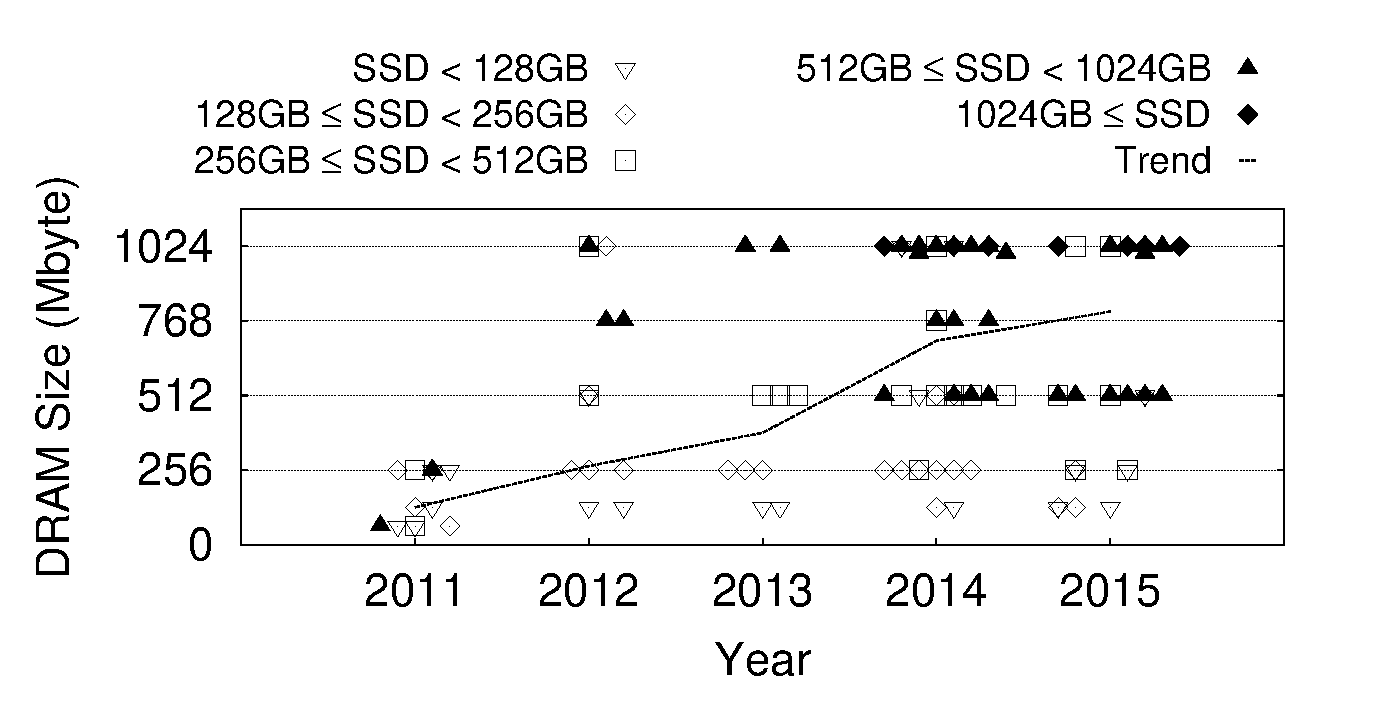
\includegraphics[width=3.2in]{./figure/dram_size.eps}
\caption{DRAM size Trend in SSDs (From 2011 to 2015)}
\label{fig:dram_size}
\end{center}
\vspace{-1.5em}
\end{figure}

The second issue is that stacking log systems generate more
severe issue called compound garbage collection---the phenomenon where
log-structured storage performs garbage collection on data that
log-structured file system already completed performing segment
cleaning. As the result of compound garbage collection, storage has to
re-write the data block that is already in the storage device and recreate
segment cleaning overhead of file system on storage. 
Compound garbage collection amplifies the volume of I/Os transferred to 
the NAND Flash memories in the SSD. This inefficient behavior 
not only degrades overall system performance but also reduces the life span of SSD device.

In this paper, we develop Unified Storage Layer (USL) to address the two
issues in exploiting the stacked log-structured systems, which are the
size of the mapping table and compound garbage collection. 
Our solution integrates address indirection layers on host and SSD into
the file system; USL reduces the overhead in managing mapping tables in
different log layers. USL resolves compound garbage collection issue
by delegating the job of device garbage collection to
file system. There are four essential building blocks in URL. The first
is disaggregate mapping scheme that allows using separate mapping
schemes for file system metadata and user data; the second is block
patching that prevents partial writes in the storage device which is
the result of misaligning file system block size against NAND page
size; the third is compound garbage collection scheme; and the last
one is Quasi-Preemptive Segment Cleaning scheme to improve the
response time in performing file system segment cleaning process.

There are three contributions in this paper: (i) USL
reduces the size of memory required to store metadata of an SSD by
1/54, (ii) USL exhibits 39$\%$ better performance than Ext4
file system, and (iii) USL resolves compound garbage collection issue
inherent in stacked log-structured system.

We modify the firmware of 843Tn SSD
\cite{ssd843tn} and F2FS to implement USL and compare the performance
with existing systems.  USL mapping scheme
allows reducing the mapping table size to 1/54 of page mapping. 
The write amplification in USL is about 26$\%$
lower and IOPS is 45$\%$ higher compared to that of base F2FS in
stacked log-structured system. 


The rest of the paper is organized as follows. Section
\ref{sec:background} describes how log-structured file system and SSDs
work, and issues stacked log system. Section \ref{sec:CompoundGC}
defines the notion of compound garbage collection problem and provides
an example to explain the problem. Section \ref{sec:USL_design} and
Section \ref{sec:USL_implementation} describes design and
implementation of Unified Storage Layer (USL), respectively. Section
\ref{sec:measuring_waf} compares analytical write amplification
between F2FS, Ext4, and USL. Section \ref{sec:experiment} shows the
performance of USL through various experiments and workloads. Section
\ref{sec:related_works} describes the related work and Section
\ref{sec:conclusion} concludes the paper.


\section{Background}
\label{sec:background}

\subsection{Segment Cleaning in Log-structured File System}

Log-structured file system is write-optimized file system
\cite{rosenblum1992design}. The file system minimizes seek overhead by
clustering the data block and the updated metadata block in proximity.
The file system is written in an append-only manner and all out-of-date
blocks are marked as invalid. The file system maintains in-memory
directory structure to locate the up-to-date version of individual file
system blocks. To minimize the disk traffic, the file system buffers
the updates and flushes them to disk as a single unit either when the
buffer is full or when \texttt{fsync()} is called.  The invalid file
system blocks need to be reclaimed to accommodate the newly incoming
writes. The process is called \emph{segment cleaning}. The segment
cleaning overhead is one of the main reasons which bar the wider
adoption of its technology since it makes the file system under
unexpected long delay\cite{seltzer1995file}.

Append-only nature of the log-structured file system is well aligned with
the update-only nature of the Flash device. A few log-structured
file systems have been proposed specifically for Flash storage
\cite{manning2010yaffs, woodhouse2001jffs, lee2015f2fs}. Amongst these file systems, only the Flash
Friendly File System(F2FS) \cite{lee2015f2fs} has successfully reached the level
of sufficient maturity and have been deployed as a commodity file system
replacing the commodity Ext4 \cite{cao2007ext4}. Let us briefly go into further
details for F2FS. Different from existing log-structured file systems,
F2FS provides finger categorization on segment types and maintains six
types of segment buffers to cluster the blocks with 
similar life time together. To reduce the garbage collection overhead,
it is important that the blocks in a segment bear similar
\texttt{hotness} \cite{rosenblum1992design, min2012sfs}. Subject to the hotness, F2FS provides three
levels of segment hotness: \emph{hot}, \emph{warm} and
\emph{cold}. The segments are categorized into two types subject to its
content: data vs.~directory. Combined together, F2FS defines six types
of segments. Fig. \ref{fig:f2fs_partition} illustrates the layout of
F2FS partitions. F2FS partitions the entire file system partition into
two, \emph{metadata} area and \emph{data} area and  maintain them
differently. Metadata area is updated in an in-place manner and the data
area is updated in an out-of-place manner. Flash device does not have seek
time overhead and, therefore, there is no need to cluster the metadata and
data block. Further, metadata blocks are updated much more frequently
than data blocks are updated. To properly accommodate the discrepancy in
access pattern, F2FS separates the region for metadata and data blocks.

F2FS allows separating the unit of write, \emph{segment}, and the unit
of erase, \emph{section}.  A section is a collection of consecutive
segments and by default the section size is one segment. This flexible
design allows F2FS to be well integrated with superblock based
SSD \cite{seong2010hydra}. F2FS adopts  greedy \cite{kawaguchi1995Flash} and cost
benefit \cite{rosenblum1992design} policy for foreground and background
cleaning, respectively.

\begin{comment}
  A log-structured file system is a append only system. All writes are
  sequential which makes it ideal for SSDs. In log-structured
  file system, an entire file system is divided with a unit called
  segment, which is a set of consecutive file system blocks. Upon
  receiving a write request, the log file system allocates a free segment
  for data and use it to append more data until the segment is
  full. Note that the size of segment varies, e.g., 8 Mbyte in NILFS2
  \cite{nilfs_segment_size}, 512 Kbyte to 1 Mbyte in Sprite-LFS
  \cite{rosenblum1992design}, and 2 Mbyte in F2FS
  \cite{f2fs_segment_size}. Note that F2FS is a fairly young log
  file system which targets to assimilate the characteristics of Flash
  memory. Recent report on F2FS \cite{lee2015f2fs} shows that its
  performance is about 3.1 times better than Ext4 \cite{cao2007ext4} on
  some workloads.
  % Jeong et al. \cite{jeong2013stack} showed that F2FS is also well suited for mobile workloads. 
  Fig. \ref{fig:f2fs_partition} illustrates the layout of F2FS
  file system partition. There are two areas in F2FS file system
  partition: Metadata area, which keeps file system related metadata and
  Main, which area keeps user generated data along with file related
  metadata (node).
\end{comment}


\begin{figure}[t]
\begin{center}
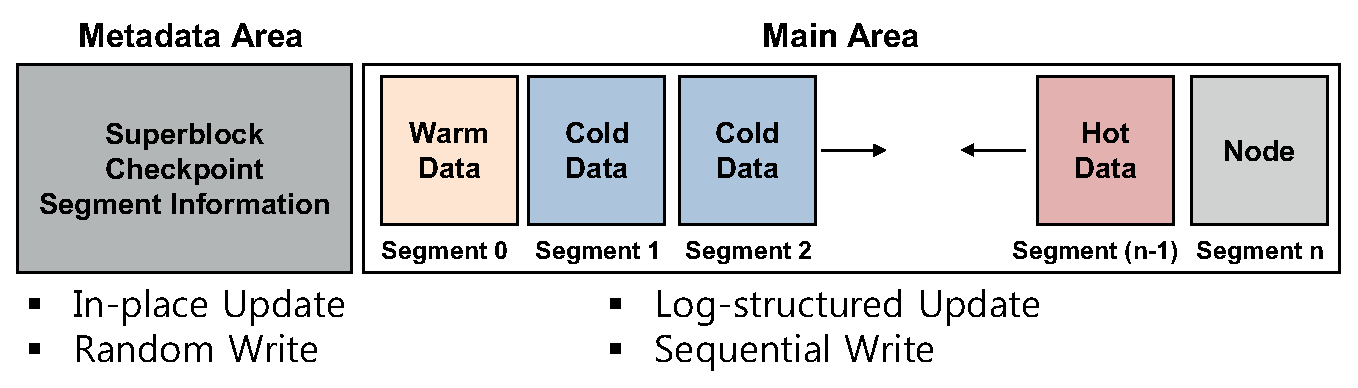
\includegraphics[width=3.2in]{./figure/f2fs_layout}
\caption{F2FS Partition Layout}
\label{fig:f2fs_partition}
\vspace{-1.9em}
\end{center}
\end{figure}


\begin{comment}
  F2FS triggers segment cleaning when the number of free segments goes
  under predefined threshold. The unit of garbage collection in F2FS
  is a section which is defined as groups of segments---by default it
  is set as one segment in a section. A victim section in a segment
  cleaning process is decided by two segment cleaning policies called
  foreground and background segment cleaning, which are base on greedy
  \cite{kawaguchi1995Flash} and cost benefit
  \cite{rosenblum1992design}, respectively. Once the victim is
  selected, valid data in the sections are copied to the current
  segment and reverts the section to free section. Note that segment
  cleaning process impedes user I/O operations because it is
  non-preemptive operation.
\end{comment}

\subsection{Garbage Collection in Flash Storage}

Garbage collection is a process of reclaiming invalid pages in the
Flash storage \cite{agrawal2008design}. Garbage collection not only interferes with the IO
requests from the host but also shortens the lifespan of the Flash
storage. A fair amount of garbage collection algorithms have been
proposed; Greedy \cite{kawaguchi1995Flash}, EF-Greedy \cite{kwon2007ef}, Cost benefit \cite{rosenblum1992design}, and etc.
Various techniques have been proposed to hide the garbage
collection overhead from the host. They include background garbage
collection \cite{smith2011garbage}, pre-emptive garbage collection \cite{lee2011semi}, and
etc. SSD controller allocates separate hardware thread for garbage
collection so that garbage collection does not interfere with IO request
from the host. Despite that numerous algorithms have been proposed since the
inception of the Flash storage, the garbage collection is still
problematic \cite{bux2010performance}.  

Garbage collection in Flash storage and the segment cleaning in
log-structured file system are essentially identical: consolidate the
valid blocks and reclaim the invalid blocks.

\begin{figure}[t]
\begin{center}
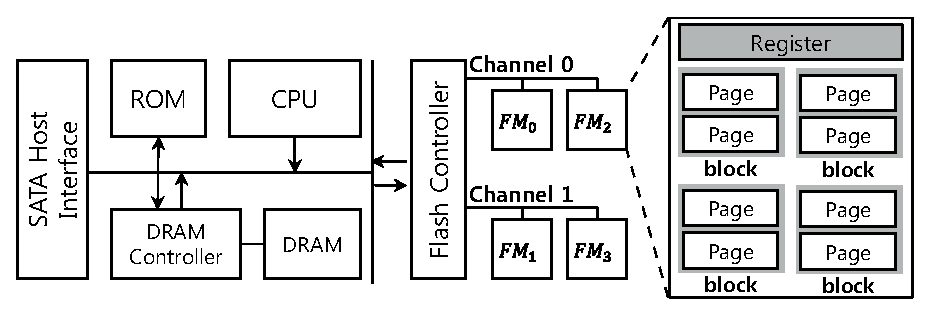
\includegraphics[width=3.2in]{./figure/ssd_internal.eps}
\caption{Block Diagram of an SSD}
\label{fig:ssd_internal}
\end{center}
\vspace{-1.9em}
\end{figure}
In multi-channel/multi-way architecture, SSD controller can perform
garbage collection in per-channel basis.
Fig. \ref{fig:ssd_internal} illustrates the architecture of an SSD with
2 channel/2 way configuration. When Flash memories in a channel are busy
with handling garbage collection process, the other channel can handle
the I/O requests. 

\begin{comment}
  Kang et al. \cite{kang2006superblock} introduced Superblock FTL for
  In multi-channel/multi-way configuration; ingenuity of Superblock
  FTL is the introduction of the notion called super-block, which is a
  group of pages with same offset in NAND blocks on each channel and
  ways. When Superblock FTL receives a write request, a empty
  super-block is allocated to store the data. This process repeats
  until there is no free pages in the current super-block. It
  naturally makes most out of multi-channel and multi-way parallelism
  of the SSD. Since the garbage collection in Superblock FTL also
  exploits super-block as a unit, SSD suffers from garbage collection
  overhead dearly because it cannot handle any of read/program
  requests.
\end{comment}

\begin{comment}

\subsection{Log-structured File System and SSD}

  Originally, log-structured file system came out to improve the random
  write performance of slow HDDs. Even though the idea of exploiting
  sequential performance of the device captured many researchers
  attention, but the fact that there is the overhead of garbage
  collection made many hesitant in adopt it in a running system.

  Behind the scene, FTL manages mapping between logical to physical addresses and takes care
  of out-of-place updates. Researchers in the field have proposed many
  different mapping schemes such as page level FTL \cite{ban1995Flash},
  Block FTL \cite{kim2002space}, and hybrid FTLs
  \cite{kang2006superblock, fast07, last08}.

  Page level FTL has been the de facto mapping
  scheme used in the industries. however, large memory footprint
  requires SSD to adopt larger DRAM memory. Fig \ref{fig:dram_size}
  shows that the size of DRAM increased considerably over the years. It
  shows that about 60$\%$ of SSDs have 512 Mbyte and 1 Gbyte of DRAM.
\end{comment}


\begin{comment}
  A reasons behind the growth of DRAM size is to reflect the increased
  size of SSD metadata such as mapping table. Instead, it can exploit block level mapping which
  is better for sequential workloads and also can significantly reduce the
  size of mapping information. A 256 Gbyte SSD
  with 4 Kbyte page and 2 Mbyte of block, the page level FTL needs 
  256 Mbyte of mapping table, but block FTL only needs to
  store 512 Kbyte of information. Since log file system is aimed for  
  generating sequential workloads, it would be ideal to match log
  file systems with SSDs, then it can exploit block level mapping.
\end{comment}

\vspace{-0.5em}

\subsection{Stacking the Logs}
Log-structured file system in its essence is well aligned with the
append-only nature of the SSD. Sequential IO request originated by
log-structured file system can greatly simplify the address mapping and
the garbage collection overhead of the underlying storage.  Recently, a
number of key-value stores exploit append-only update mechanism to
optimize its behavior towards write operations \cite{lim2011silt, ghemawat2014leveldb}. 
However, the log-structured file system for SSD  entails a number
of redundancies whose result can be disastrous. There exist majorly
three redundancies: (i) garbage collection, (ii) mapping information,
and (iii) overprovisioning area.  Fig.~\ref{fig:layered_log_system}
illustrates an example: a log-structured file system over an SSD. 

First, each layer performs garbage collection on its managing address
space. There exist redundant efforts of log-structured storage device to
garbage collect data which are already cleaned on log-structured
file system. It not only degrades the IO performance but also may shorten
the life span of the Flash storage. We call this as \emph{Compound
Garbage Collection}. The issue is discussed in Section
\ref{sec:CompoundGC} in more detail. 
Second, each layer has to manage its own metadata to keep information
for address mapping, and, as a result, larger memory is required to load
the metadata. As the capacity of SSD increases, the overhead of
maintaining the mapping information at Flash page granularity becomes
more significant. 
Third, each of the log layers needs to reserve a certain fraction of its
space, the over-provisioning area. The log-structured file system (or
SSD) sets aside a certain fraction of its file system space (or storage
space) to host the extra write operations caused by garbage
collection. Overprovisioning is an indispensable waste of the expensive
Flash storage. The total amount of overprovisioning areas for individual log
layers can be very significant. 

\begin{comment}
  Two log-structured systems stacked on top of each other is called as
  stacking log system, and an example of such system is illustrated in
  Fig \ref{fig:layered_log_system}. It shows that log file system is on
  top of Flash-based storage device. When virtual file system sends data
  down to file system, the data is recorded in the file system
  partition. When there is not enough space left in the partition, the
  file system runs segment cleaning to tidy up the invalid data. As a
  result, the file system has to send not only the data received from the
  virtual file system but also the writes generated by the segment
  cleaning.

  When the device writes the received updates on the storage medium, 
  FTL decides where to put the data. When there is not enough space in
  the storage, SSD runs garbage collection to reclaim free pages for
  incoming data. Initial write volume increases as it is passed down in
  the I/O hierarchy, which is typical in log-structured systems. And, it
  is called Write Amplification.  Larger write amplification means
  trouble for SSD because it not only has to handle more data but also
  reduces the life of the device.
\end{comment}


\begin{figure}[t]
\begin{center}
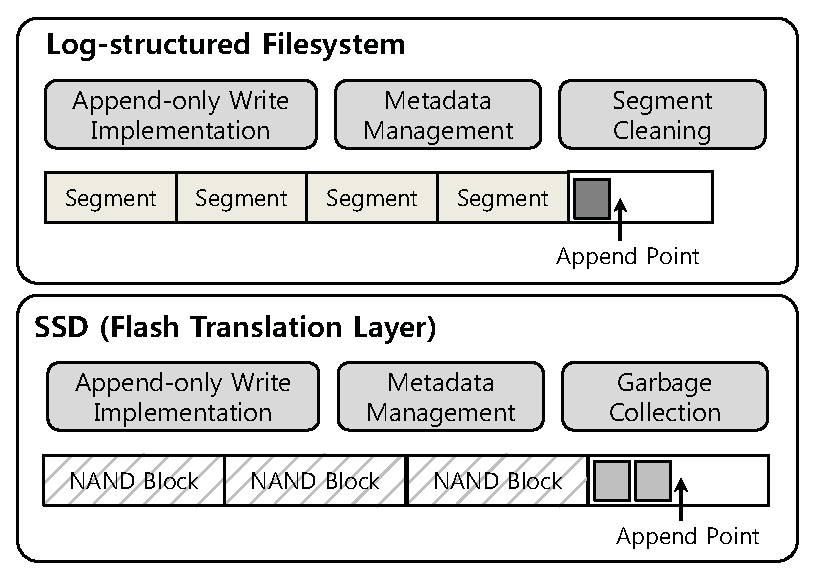
\includegraphics[width=3in]{./figure/layered_log_system}
\caption{Example of Stacking Log System}
\label{fig:layered_log_system}
\vspace{-1.5em}
\end{center}
\end{figure}


\begin{figure*}[t]
\begin{center}
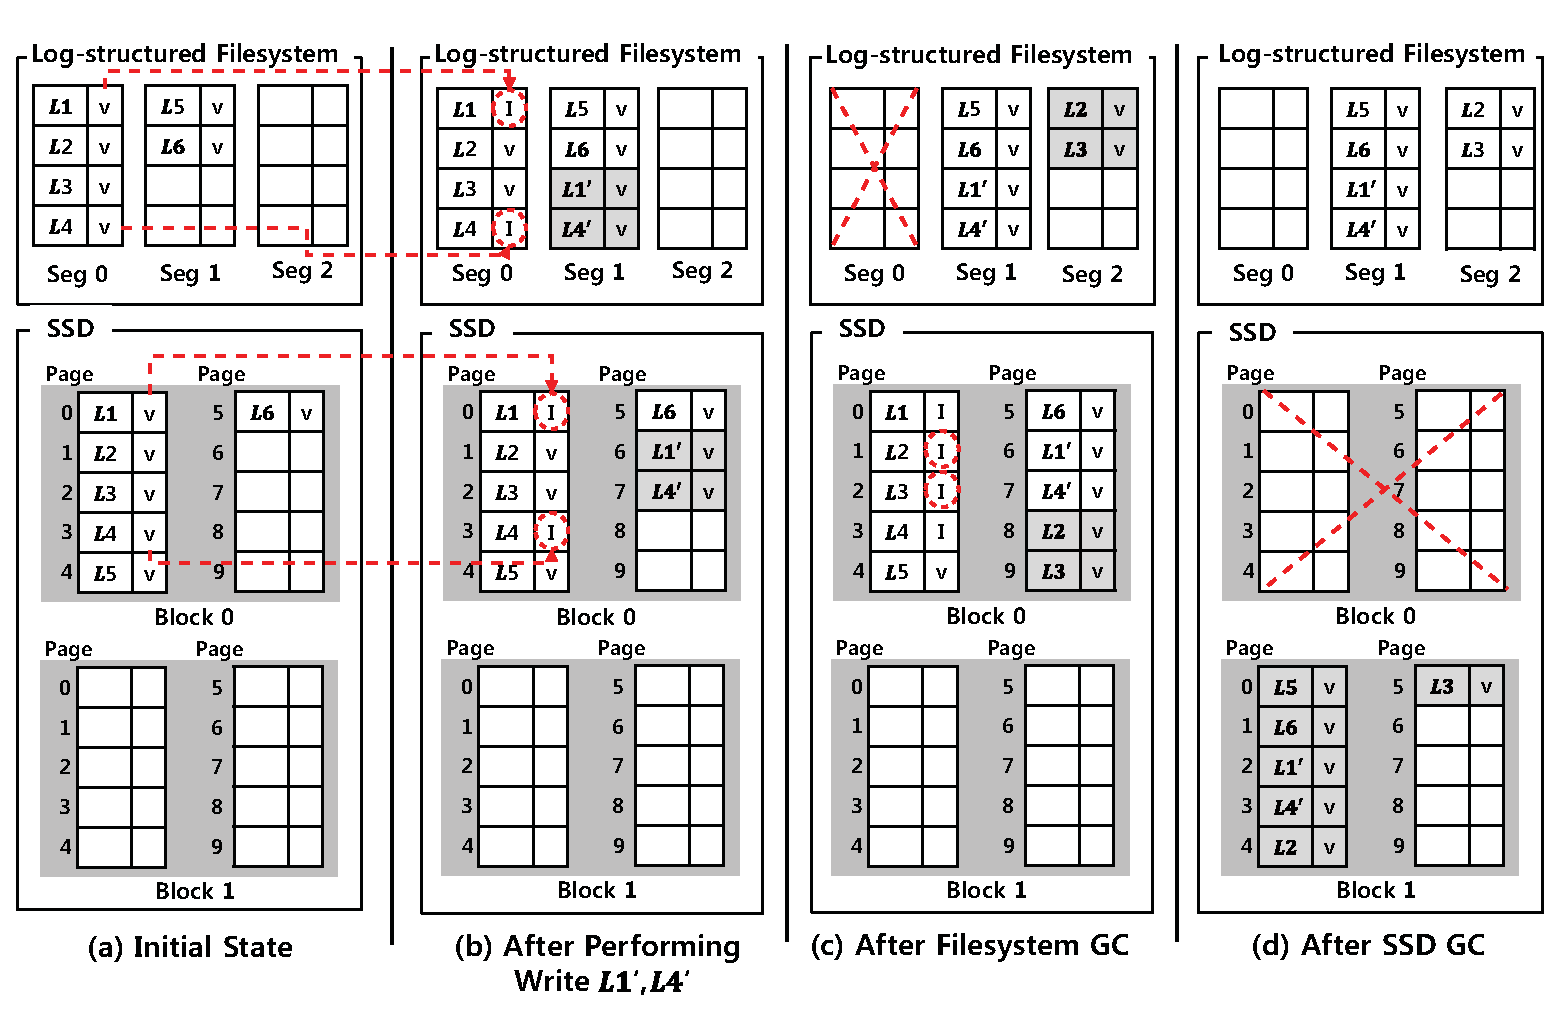
\includegraphics[width=5.7in]{./figure/comp_gc_scenario_1}
\caption{Example of Compound Garbage Collection ($Ln$ means LBA $n$)}
\label{fig:comp_gc_1}
\end{center}
\vspace{-1.5em}
\end{figure*}

\section{Compound Garbage Collection}
\label{sec:CompoundGC}

We define Compound Garbage collection as the phenomenon where the storage
level log system performs garbage collection on data blocks which are
already segment cleaned by a log-structured file system. The compound
garbage collection not only degrades the IO performance but also shortens
the lifespan of the Flash storage.

Fig. \ref{fig:comp_gc_1} illustrates a scenario of compound garbage
collection. We assume that each segment on a file system has four pages
and the file system performs garbage collection in units of
segments. The segments that are not shown in Fig.~\ref{fig:comp_gc_1}
store cold data. Each block on the SSD 
contains ten pages. The file system and the SSD perform garbage
collection when only one empty segments and only one empty block is left
on the layer, respectively. Additionally, we assume that the
SSD  is aware of the invalidated LBAs through TRIM command
\cite{shu2007data}.

$L_i$ denotes the logical page Fig.~\ref{fig:comp_gc_1} denotes the
logical page. The flag represents the state of the corresponding page; $V$ is
for valid and $I$ is for an invalid page. Initially, segment 0 holds data
pages for LBA 1 to LBA 4, and segment  
1 contains LBA 5 and LBA 6. Both segments are stored in block 0 on the
SSD. 

Fig. \ref{fig:comp_gc_1}(b) shows the state of the file system and the
SSD after $L1$ and $L4$ are updated. The updated block is appended at
the end. The flags in old pages of the file system and SSD are now set
to invalid. Upon receiving an update, the file system writes a new data on
segment 2; the file system finds that there is only one free segment
left, and thus triggers the segment cleaning process.

Fig. \ref{fig:comp_gc_1}(c) shows the status of each layer after segment 
cleaning. The file system has selected the segment 0 as the victim
segment. Valid pages in the segment 0, $L2$ and $L3$, are copied to the
segment 2. The file system notifies the changes to the storage
device. The SSD thinks that $L2$ and $L3$ are updated in the file system,
so it invalidates pages 1 and 2. Then, the SSD writes $L2$ and $L3$ on
page 8 and page 9 in block 0, respectively.  

After writing to page 8 and page 9, the SSD finds that there is only one
empty block left; thus, the garbage
collection takes a place(Fig.~\ref{fig:comp_gc_1}(d)). The block 0 is
selected as the victim.  All the valid pages in block 0 are
copied to empty block 1, and block 0 is erased and becomes free.

There are two things to note in our case study. First, the SSD garbage
collection is triggered because of the file system segment
cleaning. Second, both file system and storage system pass around $L2$
and $L3$ over and over. Compound Garbage collection problem aggravates
when garbage collection unit of upper log layer is smaller than that of
lower log system  \cite{yang2014don}.

\begin{figure*}[t]
\centering
 \subfigure[Ext4 with Page mapping SSD]{
 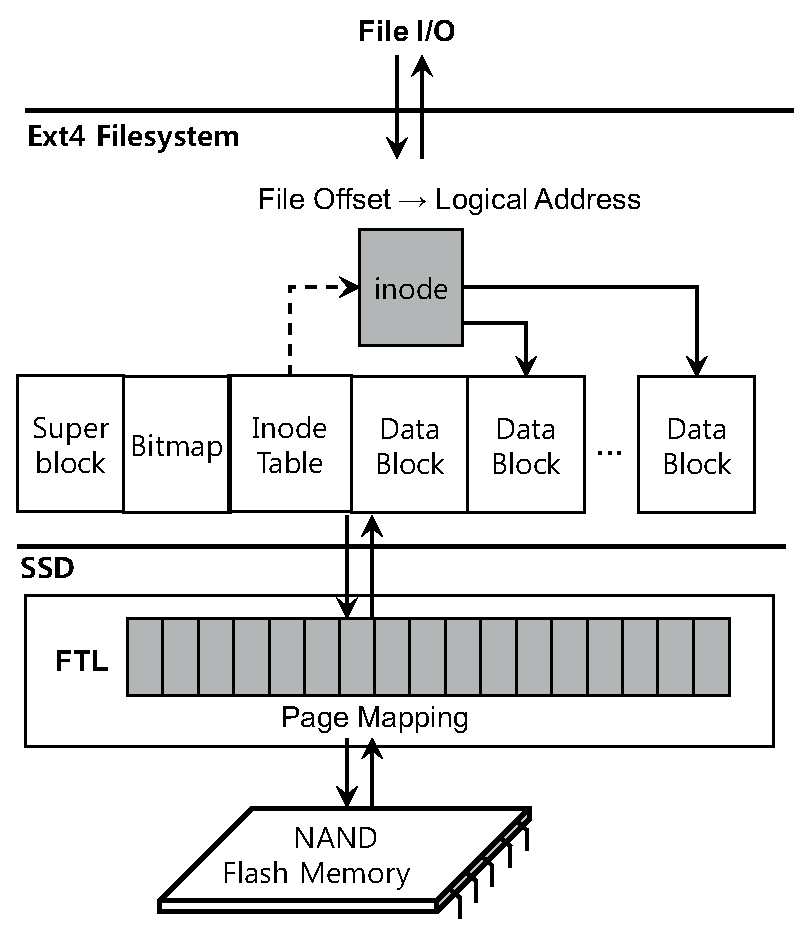
\includegraphics[width=2in]{./figure/ext4_arch}
 \label{fig:ext4_layout}
 }
 \subfigure[F2FS with Page mapping SSD]{
 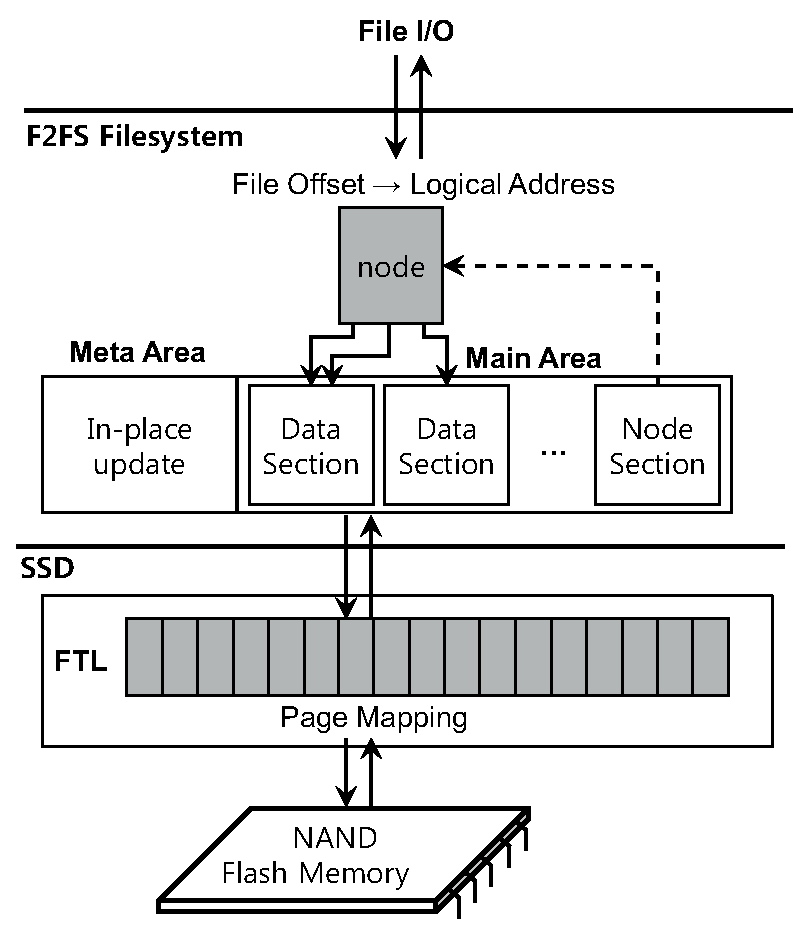
\includegraphics[width=2in]{./figure/f2fs_arch}
 \label{fig:f2fs_layout}
 }
 \subfigure[Unified Storage Layer]{
 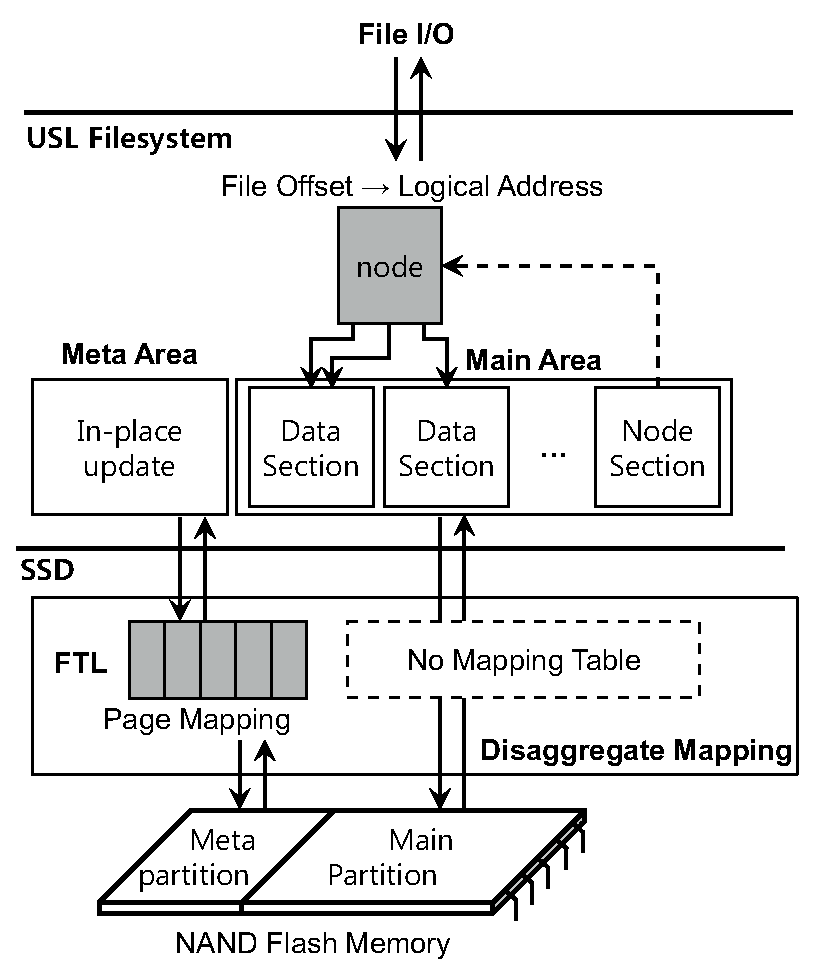
\includegraphics[width=1.92in]{./figure/usl_architecture}
 \label{fig:usl_layout}
 }
\caption{System Layout for Different File Systems and SSD Mapping
  Scheme}
\vspace{-0.5em}
\label{fig:system_layout}
\end{figure*}

\section{Design: Unified Storage Layer}
\label{sec:USL_design}

\subsection{Concept}
We propose Unified Storage Layer, \emph{USL}. It intends to address
three issues in the stacked log system: (i) Compound garbage collection,
(ii) redundant mapping information and (iii) overprovisioning
overhead. 

Unified Storage Layer consists of a log-structured file system and an SSD.
In USL, SSD exposes its physical blocks to the host. USL is directly
responsible for address mapping and garbage collection of the Flash
storage. In USL, SSD does not have its
own mapping table nor the garbage collection module. USL does not have
to reserve its own overprovisioning area. The similar file system has been
widely used in embedded device area \cite{manning2010yaffs, woodhouse2001jffs}.

YAFFS (Yet Another Flash File System) \cite{manning2010yaffs} is a
file system for a Flash memory package, and the file system manages
Logical-to-Physical mapping and garbage collection as well as
wear-leveling of the device. Although YAFFS is a log-structured
file system, it uses NAND block as the unit of garbage collection
instead of segment. Unlike USL and F2FS, YAFFS can reclaim an only
limited number of NAND blocks at each round of garbage collection
process. The mapping table in YAFFS is managed in Physical Address
Translation Tree, and as the file gets larger, the search overhead
also increases. Moreover, YAFFS is meant for NAND device and is not
for SSDs.

USL eliminates the above listed three redundancies in using
log-structured file system over SSD. In the current implementation of USL,
bad block management is left to the Flash storage.

We take advantage of the existing log-structured file system, F2FS
\cite{lee2015f2fs}. F2FS adopts in-place update for metadata region and 
out-of-place update for data region. To effectively incorporate this
file system characteristics, we develop \emph{Disaggregate Mapping} which
adopts different mapping granularity for different parts of the storage
space. Fig. \ref{fig:f2fs_partition}, there are two regions in F2FS
partition. For metadata data and data area, USL applies page mapping and
section based mapping which is to be detailed shortly, respectively.
Fig. \ref{fig:system_layout} compares different file system layouts
including in-place update file system (Ext4), log-structured file system
(F2FS), and USL. Fig. \ref{fig:ext4_layout} illustrates a
configuration of Ext4 file system, which consists of metadata and data
blocks region and each data block has the default size of 4 Kbyte. F2FS and USL
shown in Fig.~\ref{fig:f2fs_layout} and Fig. \ref{fig:usl_layout},
respectively, manages file system partition with segments and sections.

\begin{figure}[t]
\begin{center}
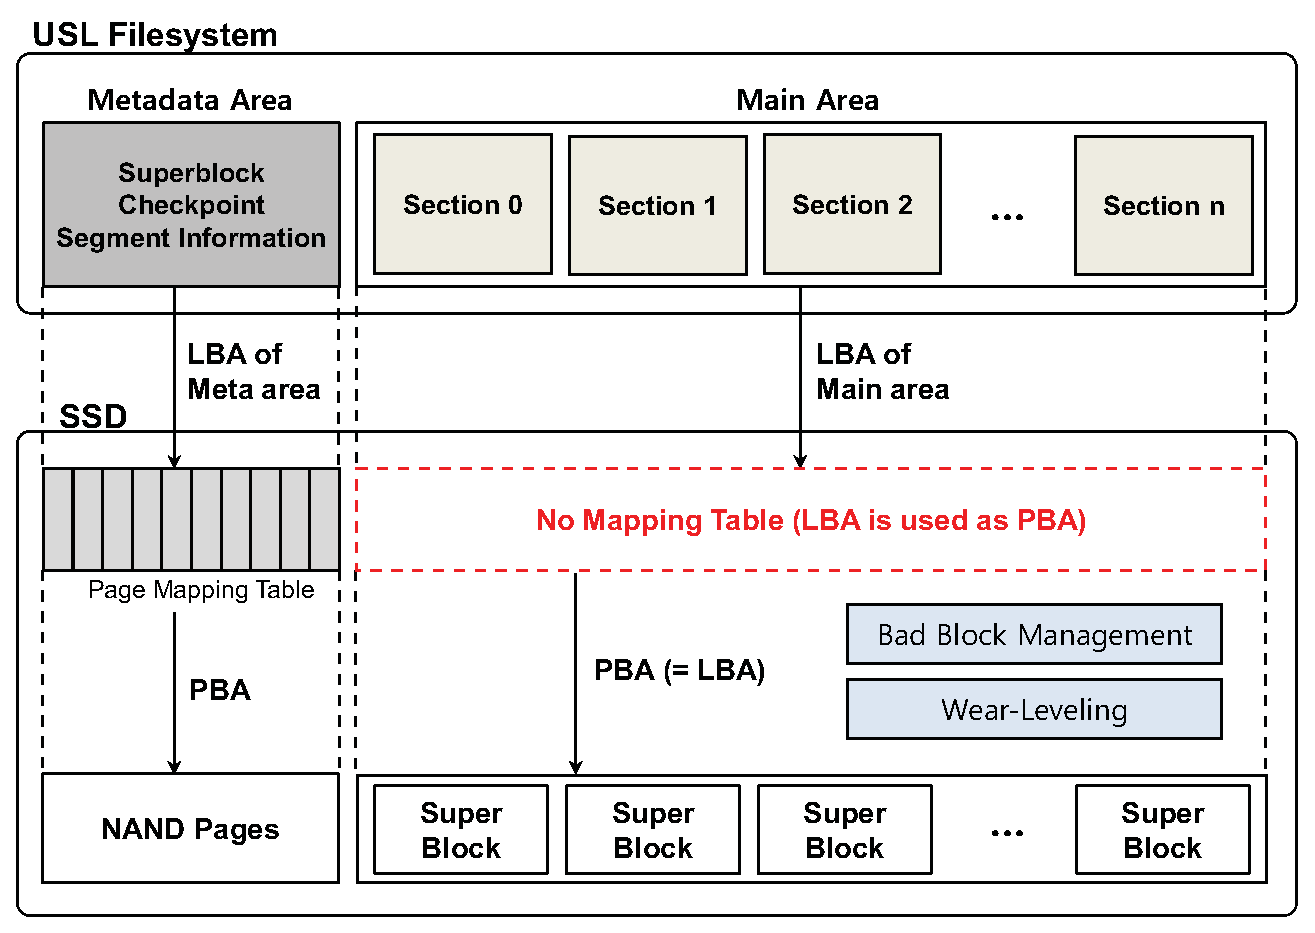
\includegraphics[width=3in]{./figure/usl_layout}
\caption{Disaggregate Mapping Layout}
\label{fig:da_mapping_layout}
\vspace{-2em}
\end{center}
\end{figure}


\subsection{Disaggregate Mapping}
\label{subsec:da_mapping}

\begin{table*}[t]
  \begin{center}
  \begin{tabular}{|c|c|c|c|c|c|} \hline
  & USL & ANViL \cite{anvil} & FSDV \cite{zhangremoving} & NVMKV \cite{nvmkv} & SDF \cite{sdf} \\ \hline \hline
  Host Map & $\times$ & $\bigcirc$ (prototype) & $\times$ & $\times$ & $\times$ \\ \hline
  Device Map & $\triangle$ (very small) & $\times$ (prototype) & $\bigcirc$ & $\bigcirc$ & $\bigcirc$ \\ \hline
  Mapping Table Size & \# of meta pages & \# of pages & $\leq$ \# of pages & \# of pages & \# of blocks \\ \hline
  Garbage Collection & Host & Device & Device & Host & Host \\ \hline
  Need of new I/O Interface  & $\times$ & $\bigcirc$  & $\bigcirc$ & $\times$ & $\bigcirc$ \\ \hline
  Over-provisioning of Storage & $\triangle$ (very small) & $\bigcirc$ & $\bigcirc$ & $\bigcirc$ & $\times$ \\ \hline
  Target Workload & General & General & General & Key-Value Store & Specific Server \\ \hline
  \end{tabular}
  \end{center}
  \caption{Comparison between USL and other systems}
  \label{tab:compare_usl}
\end{table*}

The crux of USL is to
manage LBAs with \emph{Disaggregate Mapping}, which is a mapping
specifically tailored to accommodate two different I/O characteristics:
small random writes and large sequential writes. 
Fig.~\ref{fig:da_mapping_layout} schematically illustrates the storage
and file system layouts for Disaggregate Mapping. 
In Disaggregate Mapping, USL directly manages the main area of the
file system with section level mapping granularity. It delegates mapping
of metadata area to SSD. Metadata area needs to be managed with page
mapping. F2FS manages the main area in log-structured manner and the
unit of a write is \emph{section}. This characteristic allows a USL to
use large mapping granularity in managing the Flash storage. It
significantly reduces the mapping table overhead. In USL, the section
size is aligned with the superblock size of an SSD. The superblock size
is the block size $\times$ number of channels. In our settings, the page
size is 8 Kbyte and section size is 256 Mbyte. The SSD
Firmware makes the decision over received LBAs. If they are for metadata
area, the firmware directs them to page mapping managed region of the
device; if LBAs within the range of main area is received, the firmware
recognizes them as PBAs. 

USL successfully addresses the three redundancies in stacked log. 
First, it eliminates the redundant mapping tables. Mapping information
for metadata area and main area are harbored by Flash storage and the
host, respectively. More importantly, the host maintains the mapping
table in super block granularity, which reduces the mapping table size
to 1/256. For 4 Tbyte SSD, legacy page mapping requires
4 Gbyte of DRAM for mapping table. USL reduces it to 9 Mbyte. 


Second, it eliminates the possibility of compound garbage
collection. Third, since the SSD is free from garbage collection in the
main area, it removes most of the overprovisioning significantly
reduces the volume of wasted space. In order for USL to exploit 
disaggregate mapping scheme, file system needs to understand the page and
block size of the underlying SSD  and the SSD needs to be informed about
the layout of the file system in USL. The negotiation takes in place when
the file system is first formatted on the storage device. 


\subsection{Garbage Collection}
In USL, the filesystem is responsible for consolidating the valid
filesystem blocks and reclaiming the invalid blocks. The individual
filesystem blocks are statically bound to physical NAND
blocks. Consolidating the valid filesystem blocks due to segment
cleaning physically migrates the corresponding NAND pages.
USL runs segment cleaning when the number of free segments is below the
threshold. Current implementation of USL adopts F2FS filesystem. USL
adopts two types of segment cleaning: cost benefit segment cleaning
\cite{rosenblum1992design} which runs in idle time and greedy segment
cleaning \cite{kawaguchi1995Flash}. 

\begin{figure}[t]
\centering
 \subfigure[Non-preemptive Segment Cleaning]{
 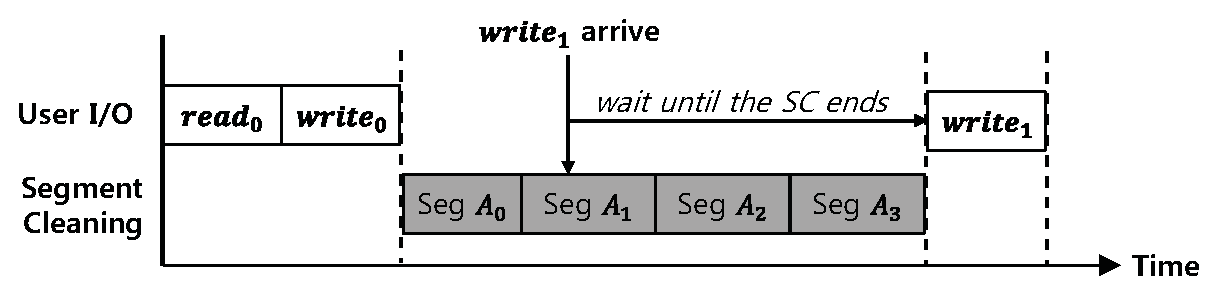
\includegraphics[width=3.4in]{./figure/preemptive_sc_1}
 \label{fig:non_preemptive}
 }\hspace{-1.3em}
 \subfigure[Preemptive Segment Cleaning]{
 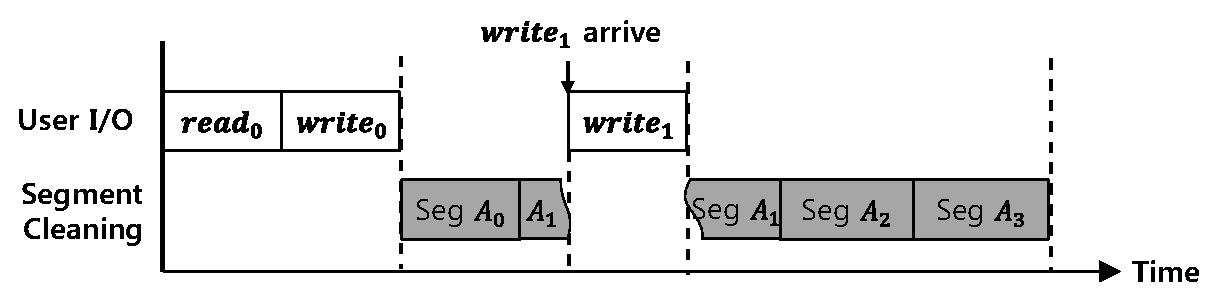
\includegraphics[width=3.4in]{./figure/preemptive_sc_3}
 \label{fig:quasipreemptive}
 }\hspace{-1.3em}
 \subfigure[Quasi-Preemptive Segment Cleaning]{
 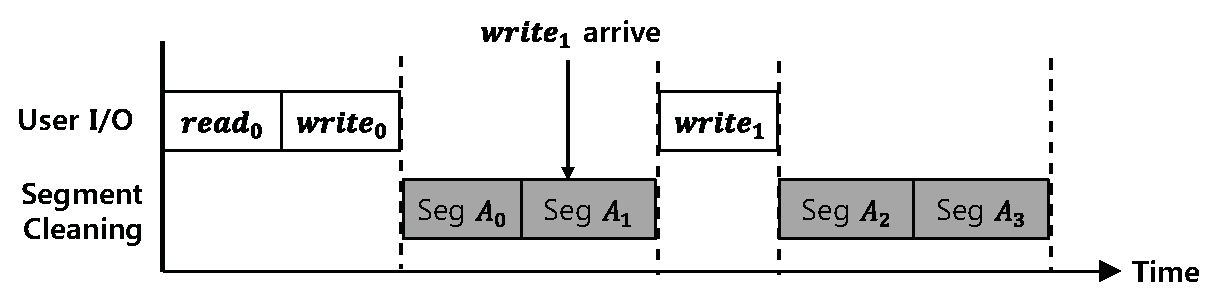
\includegraphics[width=3.4in]{./figure/preemptive_sc_2}
 \label{fig:preemptive}
 }
 \caption{Different Segment Cleaning Behaviors}
 \vspace{-1.5em}
 \label{fig:quasi_sc}
\end{figure}

The unit of segment cleaning in USL is a \emph{section}, and we
configure it to match the erase unit of an SSD. Segment cleaning
consolidates all segments in a section.  For example, the SSD
used in the experiment has superblock of 256 Mbyte. The segment cleaning
latency can be prohibitively large especially when it interferes with
the IO request. We develop Quasi-Preemptive Semgent Cleaning scheme to
reduce the  response time of segment cleaning. After each segment is
cleaned, the USL checks if there is any outstanding IO. If there is
pending user I/O, Quasi-Preemptive Segment Cleaning preempts current
segment cleaning opeartion and serves the host user I/O. 

Qausi-preemptive Segment Cleaning adopts the algorithm proposed by
\cite{lee2011semi}. 
{\color{red}
Assume that the user I/O is for the blocks in the victim section.
To copy the valid data from the victim section, the data 
will be stored in the page cache. Then, the read request gets hit 
from the page cache. 
When a read request preempts segment cleaning and requests a data
on the victim section that is not yet copied, then Quasi-Preempitve
Segment Cleaning uses the data in the page cache, instead of rereading
from the victim section, to write onto the section that the segment
cleaning is using.
On the other hand, when USL receives update request on the victim section 
and the valid data in the victim section is yet to be copied onto the 
free section, then Quasi-preemptive segment cleaning invalidates the 
data in the storage and takes the user data as the valid data and 
writes it to the free section. --> 모든 경우가 다 고려되지 않았다.}

Fig. \ref{fig:quasi_sc} illustrates an example of Non-preemptive,
Pre-emptive, and 
Quasi-Preemptive Segment Cleaning with a victim section, A. There are
four segments, A0 to A3, in the section. While segment cleaning segment
A1, the system received user I/Os. 
Once Non-preemptive Segment Cleaning (Fig. \ref{fig:quasi_sc}(a))
runs, it never gets interrupted, and all I/O requests receivd during
the cleaning process are serviced after the segment cleaning is
comleted. Thus, Non-preemptive Segment Cleaning delays the user I/O
response time. Preemptive Segment Cleaning
(Fig. \ref{fig:quasi_sc}(b)), on the other hand, stops the job and
handles the user I/Os immediately. Although it provides better
response time, but there is overhead of continously checking the user
I/O requests. Another issue in this approach is that user data may be
placed in the same block as valid pages from the victim blocks,
breaking the locality of the user data. 

Quasi-Preemptive Segment Cleaning (Fig. \ref{fig:quasi_sc}(c)) 
checks for any outstanding I/Os 
after each segment in the victim section is cleaned. If there is
requests pending, the system preempts current segment cleaning
opeartion and serves the write request. When the request is completed,
the system resumes preemted segment cleaning opeartion and cleans
segment A2 and A3. 


\begin{figure}[t]
\begin{center}
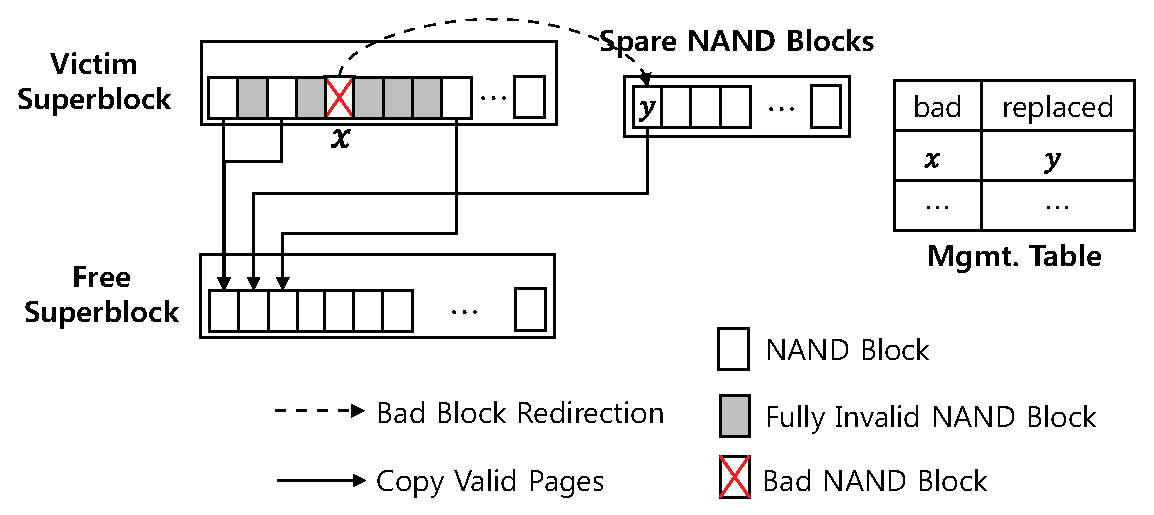
\includegraphics[width=3.5in]{./figure/bad_block_management}
\caption{Segment Cleaning with Bad Block Management}
\label{fig:bad_block}
\vspace{-2em}
\end{center}
\end{figure}

\subsection{Bad Block Management}


In USL, SSD is responsible for bad block management. An SSD sets aside a
set of NAND Flash blocks as a spare area \cite{chow2007managing}. Spare area is not
visible to the host. SSD provides a bad block management module with bad block 
indirection table. Bad block indirection table consists of a pair of
$<$physical block number, spare block number$>$. Physical block number
denotes the physical block number of the bad block. Spare block number
is the physical block number of the spare block where the IO request for
the bad block is redirected to. In segment cleaning, all the valid
blocks are consolidated to the newly allocated segment. The replacement
block allocated for the bad block is also migrated to the newly
allocated segment. After the replacement blocks is copied to the newly
allocated segment, the respective bad block mapping table is reset.
Fig. \ref{fig:bad_block} shows how the bad block management layer in SSD
interacts with segment cleaning.


\subsection{Comparison}

A few works proposed that the host holds the
responsibility to manage and modify SSD metadata to improve the
performance of the storage \cite{anvil, nvmkv, sdf}, and reduces the
size of metadata in host or device significantly
\cite{zhangremoving, nvmkv}. Table \ref{tab:compare_usl} shows that
USL has a number of advantages over existing schemes. The size of
the mapping table in USL is small, and unlike FSDV \cite{zhangremoving},
the size is fixed which reduces the management overhead. In USL,
over-provisioning area of an SSD need not be large 
because garbage collection is only performed on small area for
storing filesystem metadata. More importantly, USL does not introduce
any new I/O interface to the system; instead, it makes use of
existing ones. Finally, unlike NVMKV \cite{nvmkv} and SDF \cite{sdf}
which targets specific workloads, USL is not limited to a particular
workloads or systems.

{\color{red} Table \ref{tab:compare_usl} summarizes the efforst
\cite{anvil, zhangremoving, nvmkv, sdf}. ANViL \cite{anvil} provides
interface to host system that allows modifying logical-to-physical
mapping information in device. The host system utilizes the interface to
remove redundant data write operations. FSDV \cite{zhangremoving}
modified inodes of filesystem to point physical addresses directly which
allows dynamically reducing the mapping table size. NVMKV \cite{nvmkv}
replaced operations for key-value store with FTL commands such as atomic 
multiple-block-write, p-trim, exist, and iterate which made it possible
to remove in-memory metadata for key-value store and also to reduce
write amplification considerably. One other interesting work that
improves the performance of Flash based storage is SDF (Software defined
Flash) \cite{sdf}. In this scheme, host system controls Flash memories
in each Flash channel 
of the device. Thus, over-provisioning area of SSD is entirely open to
the user, and the software can exploit the raw bandwidth of the Flash
memory.}

Table \ref{tab:compare_usl} summarizes the efforst \cite{anvil, zhangremoving, nvmkv, sdf}.
ANViL \cite{anvil} provides address remapping interface to the host 
system that allows modifying logical-to-physical mapping information in device. The 
host system은 address remapping을 통해 다수의 logical address가 physical 
address를 share 하도록 하거나, physcical address를 가리키는 logical address를
변경함으로써, Volume Snapshots, Data Copy, Data Move 등을 데이터 쓰기 동작 없이
처리할 수 있다.
FSDV \cite{zhangremoving} modified inodes of filesystem to point physical 
addresses of an SSD directly. After updating the inode, the device removes 
the corresponding mapping table entry which allows dynamically reducing 
the SSD mapping table size.
NVMKV \cite{nvmkv} replaced operations for key-value store with FTL 
commands such as atomic multiple-block-write, p-trim, exist, and 
iterate which made it possible to remove in-memory metadata for 
key-value store. NVMKV는 이와 같은 방식으로 key-value store와 FTL의
중첩으로 발생할 수 있는 Compound Garbage Collection 문제를 해결하고, 
reduce write amplification considerably.
One other interesting work that improves the performance of Flash 
based storage is SDF (Software defined Flash) \cite{sdf}. SDF exposes 
the internal Flash channels to host as individual block device.
Each channel engine manages its own block mapping table, bad block management
and wear-leveling. The host system take charge of the garbage collection of the
Flash memory. Thus, over-provisioning area of SSD is entirely open to
the user.

\section{Implementation}
\label{sec:USL_implementation}

\begin{comment}
The file system layer in USL plays two important roles. First, it has
to persistently store the user data in the storage device. Second, it
has to handle garbage collection on main area and send a set of empty
section numbers acquired from segment cleaning process to
storage. Upon receiving the section numbers, the device makes the
corresponding NAND blocks as empty blocks. Therefore, there is no need
to run garbage collection for the NAND blocks belonging to main area but to erase
the target blocks that the file system requested.

Four parts of F2FS is modified to meet the requirements of USL
file system. First, we introduce patch manager to avoid partial writes and second, 
we modified write policy of the file system. Third, we
modified file system formatting tool. Finally, we added a mechanism
to transfer section numbers reclaimed by segment cleaning to USL
storage device.
\end{comment}

\subsection{Block Patching}

\begin{figure}[t]
\begin{center}
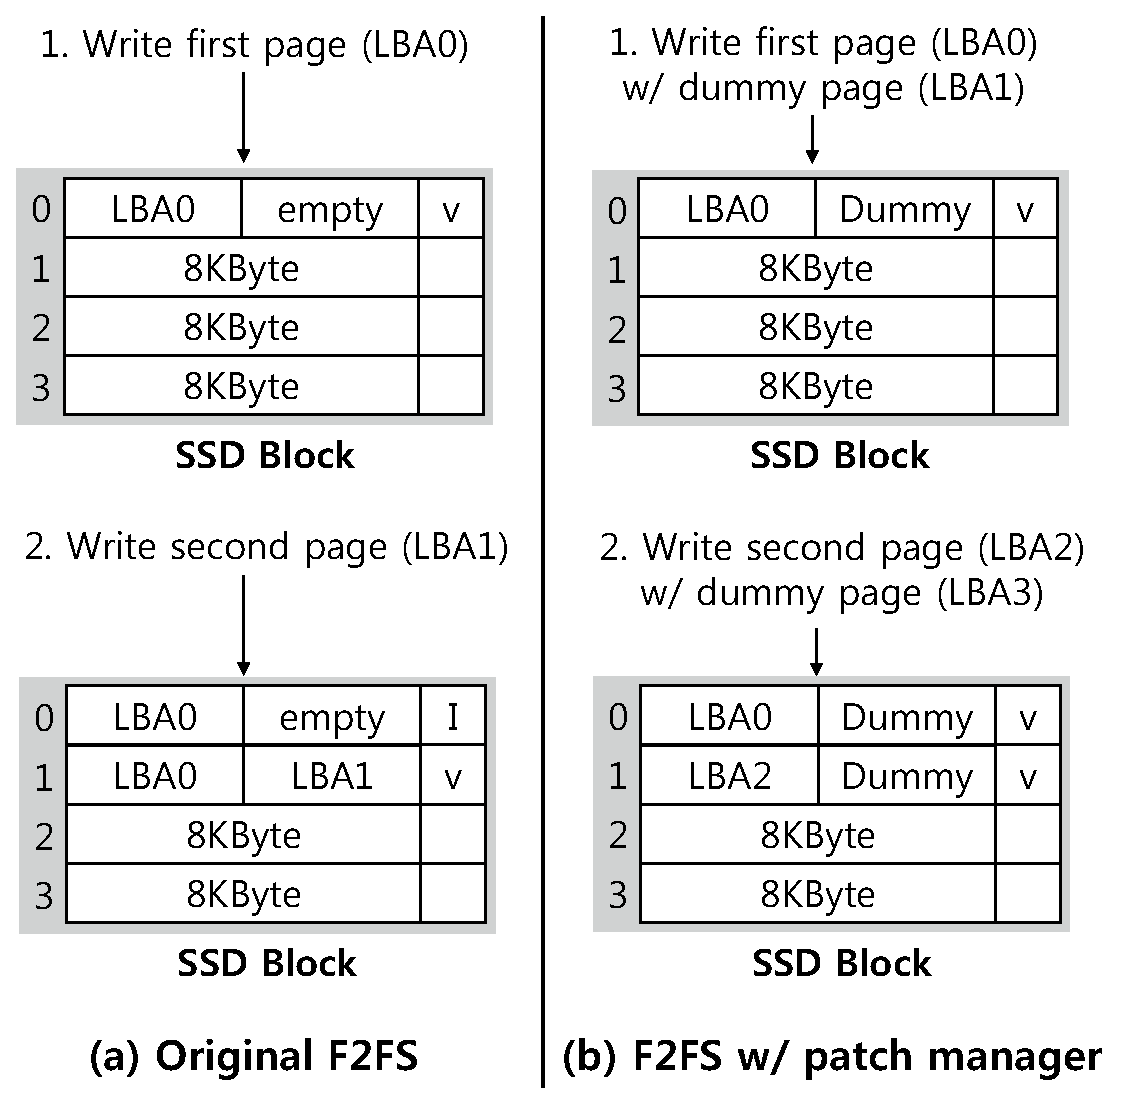
\includegraphics[width=3in]{./figure/patch_manager_ex}
\caption{Two-page Write Behavior with and without Patch Manager}
\label{fig:patch_manager_ex}
\end{center}
\vspace{-1em}
\end{figure}


File system block size is 4 Kbyte, whereas the unit size of an SSD
varies from 4 Kbyte to 16 Kbyte, depending on manufacturers. The
filesystem IO unit size is not aligned with the Flash page size. SSD
firmware is responsible for handling this discrepancy through request
merge \cite{kim2013partial}, sub-page mapping \cite{qin2011mnftl}, read-modify-write
\cite{agrawal2008design} and etc. In USL, physical Flash page is directly exposed to
host and the host filesystem need to take the responsibility of
resolving this misalignment. We develop \emph{Block Patching} for this
purpose.

Fig. \ref{fig:patch_manager_ex}(a) illustrates an issue in F2FS. Each
Flash page can store upto two filesystem blocks. To write LBA 0, F2FS
needs to perform filesystem level read-modify-write with dummy content
padded in the latter half of the Flash page. Subsequent write request
for LBA 1 entails that the LBA 0 and LBA 1 are programmed into a newly
allocated Flash page, page 0 invalidating the Flash page
0. Read-modify-write accompanies significant overhead.

We develop \emph{Block Patching} to address the overhead of
Read-modify-write in USL. When the write request size from filesystem is
not aligned with the NAND Flash page size, USL pads free page cache
entry (4 Kbyte) to the write request to make its size aligned with the
Flash page size. The filesystem needs to allocate additional filesystem
block to accommodate the padded page cache entry. While the padded page
cache entry is not reflected in the file size, it consumes an additional
filesystem block.


We introduce Patch Manager in USL filesystem layer to mandate each write
requests be aligned with the page size of the
storage (Fig. \ref{fig:patch_manager}). The patch manager allocates an
empty page from page cache and concatenates it with original write
request. 

\begin{comment}
  USL file system manipulates bio structure to form a request for the
  storage. But, before sending it to the storage, the file system sends
  it to patch manager to check whether the request is aligned with the
  page. If it is aligned, then it simply returns bio structure; and, if
  it is not aligned with the page size, then patch manager adds a dummy
  page and makes the length of the request aligned with the page size.
\end{comment}

\begin{figure}[t]
\begin{center}
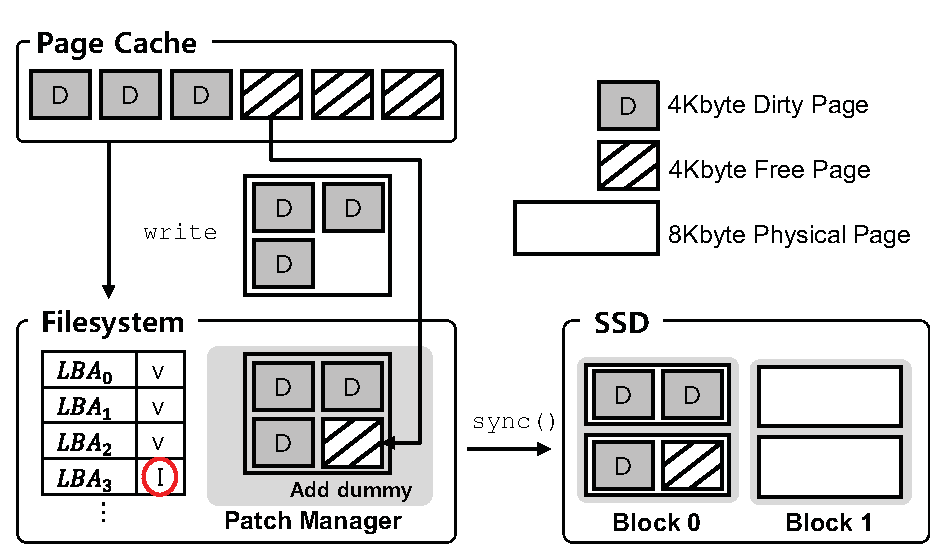
\includegraphics[width=3in]{./figure/patch_manager}
\caption{Block Patch Manager}
\label{fig:patch_manager}
\vspace{-1.5em}
\end{center}
\end{figure}


Fig. \ref{fig:patch_manager_ex}(b) shows how patch manager works in
USL. When the IO size is less than the Flash
page size, the patch manager adds dummy 4 Kbyte page along with LBA 0 and
sends it to storage in USL. The storage device assigns LBA 1 as the
dummy data and programs all the data on page 0. When
the filesystem receives a write for LBA 1, USL filesystem assigns
it to next logically consecutive address, which is LBA 2. Since the
request for LBA 2 is also not aligned, patch manager also adds dummy
page to the request and writes the request in page 1. Since a dummy
page does not contain any useful data, we mark it as invalid to let
segment cleaning reclaims the page.

Block Patching comes at the cost of additional storage space
consumption. According to our experiment, Block Patching accompanies only
3$\%$ dummy pages under 4 KByte buffered random write since few of the
filesystem writes  actually consist of a single filesystem block.


\subsection{Disabling Threaded Logging in File System}


F2FS dynamically switches between in-place update and append-only update
policy in writing the data blocks to the storage. Being essentially a
log-structured filesystem, F2FS updates the filesystem in in-place
manner when the filesystem utilization is high, \emph{threaded
logging} \cite{oh2010optimizations}. This is to avoid the expensive
foreground segment cleaning from occurring too frequently. 

USL maintains the address mapping in section granularity and it does not
allow that individual filesystem blocks are relocated to different
position. In order to guarantee that writes to main area are with only
sequential writes and can be relocated at section granularity, 
we disabled the use of threaded logging in USL filesystem. Disabling the
threaded logging causes USL to perform segment cleaning repeatedly when
the filesystem is in high utilization. We compared the performance of
USL and threaded logging in a filesystem under high utilization (Section
\ref{subsec:remove_gc_overhead}) and show that garbage collection policy
of USL outperforms F2FS with threade logging.

\subsection{Integrating the Filesystem and Storage}



\begin{figure}[t]
\begin{center}
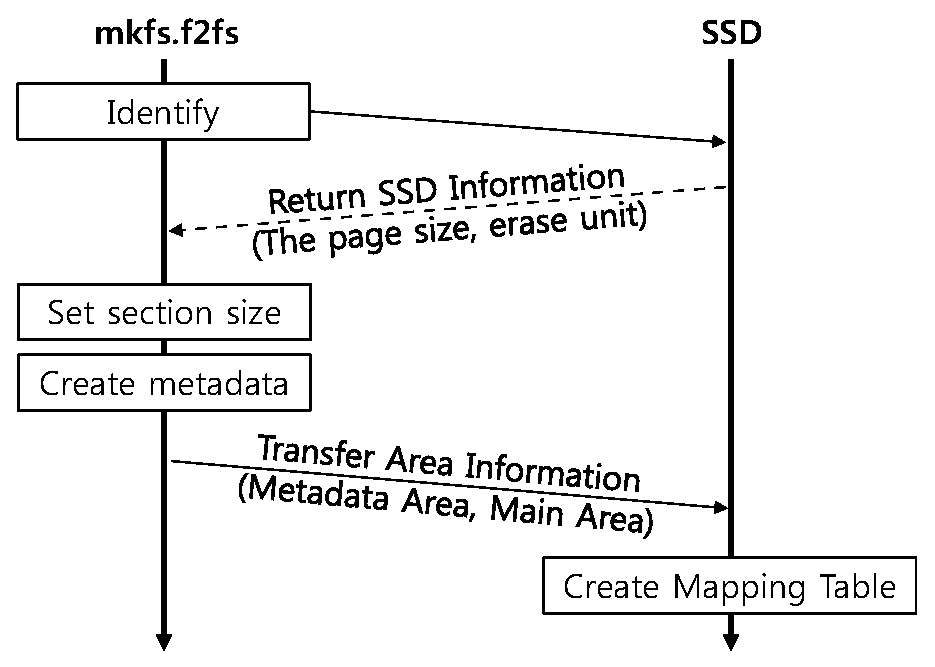
\includegraphics[width=2.5in]{./figure/formatter.eps}
\caption{Communication between mkfs.f2fs and SSDs}
\label{fig:formatter}
\end{center}
\vspace{-1.9em}
\end{figure}

The objective of Unified Storage Layer is to eliminate all the
redundancies in stacking the log-structured filesystem over the Flash
storage yielding tight integration of storage layers. In USL, the
filesystem and the storage exchanges and shares a few critical
information to make this possible. 
The storage informs the capacity, the Flash page size, and the erase
unit size to the host. Then, the host informs the storage about the size
of the metadata which it needs to maintain. The storage uses the
information to define the regions for metadata and main area of the
filesystem on the storage. We modified f2fs-tools \cite{f2fs_tools} to
acquire the information and exploit them in USL, and added new fields to
store erase unit and the size of the page of the storage in
\texttt{f2fs-tools}.  

Fig. \ref{fig:formatter} illustrates how mkfs.f2fs and SSD are sharing
its information. The phase is completed in three steps: (i) In the
beginning of filesystem format, USL device acknowledges with its page,
erase unit, and storage capacity to the filesystem, (ii) the filesystem
sets the  size of a section, creates metadata and main area, and returns
the area  information to USL storage device, and (iii) the storage
device  initializes metadata area with page mapping table and let main
area be  managed by the filesystem. 


\begin{comment}
  Theses information is transferred to each other at file system
  format time.   
  The size of metadata in USL file system depends on the capacity of the
  storage. As soon as the capacity is made known to the file system,
  it creates a file system partition and passes down the region for
  metadata and main area to the storage

  In the metadata area, F2FS keeps superblock which holds file system
  partition information,
  checkpoint for file system recovery, segment information table that
  records validity and other information about segments, and node
  address table that keeps account of file related metadata. 
  After formatting, USL file system has segment cleaning unit aligned with
  garbage collection unit of the storage, and patch manager can send
  page aligned write requests to the storage.
\end{comment}

\begin{comment}
  \begin{figure}[t]
  \begin{center}
  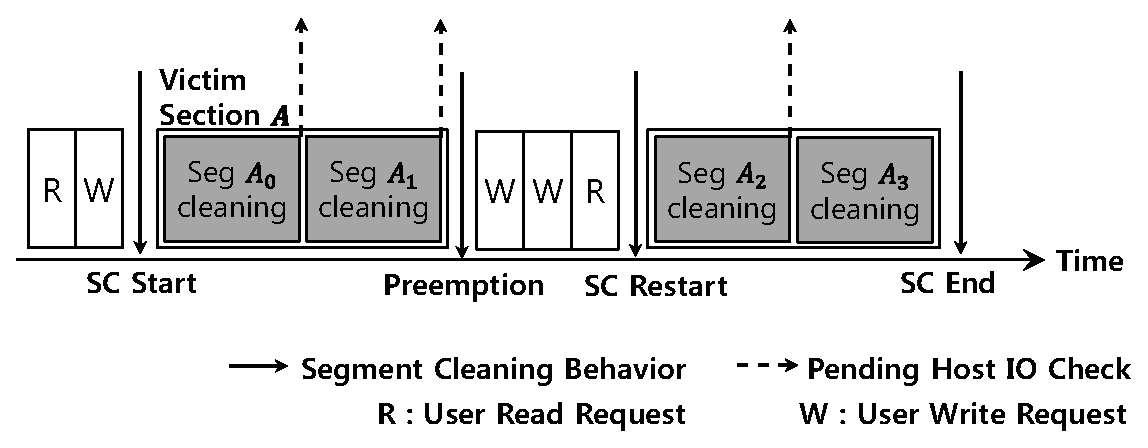
\includegraphics[width=3.2in]{./figure/preemptive_sc}
  \caption{Quasi-Preemptive Segment Cleaning Behavior}
  \label{fig:quasi_sc}
  \vspace{-1.5em}
  \end{center}
  \end{figure}
\end{comment}


\section{Experiment}
\label{sec:experiment}

\subsection{Experiment Setup}
\label{subsec:exp_setup}

\begin{comment}
  \begin{table}[h]
  \begin{center}
  \begin{tabular}{|c|c|c|c|} \hline
  		     & F2FS	& Ext4	& USL 		\\ \hline\hline
  File System	& F2FS	& Ext4	& Unified FS	\\ \hline
  SSD Mapping	& Page	& Page	& Disaggregate	\\ \hline
  \end{tabular}
  \end{center}
  \caption{System Information (File System and SSD Mapping Scheme)}
  \label{tab:system_info}
  \end{table}
\end{comment}

We compare the performance of USL against F2FS and in-place update
file system, Ext4, on Linux Kernel 3.18.1. USL uses disaggregate
mapping, and F2FS and Ext4 use page mapping SSD. 
We used 
Samsung SSD 843Tn\cite{ssd843tn} for experiments, and modified its
firmware to implement USL. 
To use disaggregate mapping on the device, we disable SSD garbage collection
in the main area, and use the information given by the mkfs.f2fs to bind
the logical address to the physical address. The firmware manages metadata 
area with page mapping table and SSD garbage collection only works for
metadata area.

Table \ref{tab:ssd_info} shows
the specification of the host system and SSD 843Tn used in the performance
evaluations. The SSD performs
garbage collection in units of superblock with size of 256 Mbyte where
superblock is a group of NAND blocks with same block number in an array of
Flash memories in channels and ways.

We use Filebench\cite{filebench} benchmark tool for the performance test.
Filebench generates a pre-defined synthetic workloads and we
make use of two workloads; fileserver, varmail. Table \ref{tab:filebench}
shows the summary of the each filebench workload.


% Table \ref{tab:system_info} summarizes the system information. 
\begin{comment}
  Since SSDs are sensitive to test environment, we create a precondition
  prior to performing any experiments. Detailed steps in the preparation
  is described in each experiments. 
\end{comment}

\begin{table}[t]
\begin{center}
\begin{tabular}{|c|p{5cm}|} \hline
\multirow{4}{*}{System} & CPU: Intel i7 @3.40GHz \\ 
& Memory:  8 Gbyte					\\ 
& OS: Ubuntu 14.04					\\ 
& Kernel: Version 3.18.1				\\ \hline
\multirow{4}{*}{Storage} & Capacity: 256 Gbyte (include 23.4 Gbyte overprovisioning) \\ 
& Page size: 8 Kbyte				\\ 
& Block size: 4 Mbyte				\\ \hline
\end{tabular}
\end{center}
\caption{Host system and storage (Samsung SSD 843Tn \cite{ssd843tn})}
\vspace{-1.5em}
\label{tab:ssd_info}
\end{table}

\begin{table}[t]
\begin{center}
\begin{tabular}{|c|c|c|c|c|c|} \hline
  		     & Files	& File size & Threads & R/W   & fsync 		\\ \hline\hline
  fileserver	& 80,000	& 128 KB	   & 50	    & 33/67 & N\\ \hline
  varmail 	& 8,000	& 16 KB     & 16	    & 50/50 & Y\\ \hline
\end{tabular}
\end{center}
\caption{Summary of Filebench Workload}
\vspace{-1.5em}
\label{tab:filebench}
\end{table}

\begin{table}[t]
\begin{center}
  \begin{tabular}{|c|r|} \hline 
                         & Mapping Size       \\ \hline\hline 
Page mapping             & 256 Mbyte          \\ \hline 
FSDV\cite{zhangremoving} & Less than equal to 256 Mbyte  \\ \hline 
Hybrid mapping (LAST \cite{last08}) & 4 Mbyte \\ \hline 
Disaggregate Mapping     & 1 Mbyte            \\ \hline
\end{tabular}
\end{center}
\caption{Size of Mapping Table (256 Gbyte SSD)}
\vspace{-2em}
\label{tab:meta_size}
\end{table}

\subsection{Mapping Table Size}

Table \ref{tab:meta_size} compares the size of mapping tables in 
Page mapping, FSDV \cite{zhangremoving}, Hybrid mapping \cite{last08},
and Disaggregate mapping.
Page mapping uses 256 Mbyte of memory when disaggregate mapping of USL uses
only 1 Mbyte. Although page mapping has large memory footprint, its
most valuable characteristics is that data can be placed in any
available places in the storage. However, as the size of SSDs is
increasing, merits in using page mapping are becoming less
appealing. For example, for 1 Tbyte and 4 Tbyte SSD with 4 Kbyte as
the page size, the memory space required to store the mapping table
information is 1 Gbyte and 4 Gbyte, respectively.

File System De-Virtualizer, FSDV \cite{zhangremoving}, makes
file system point to a physical address in an SSD, and the pointed entry
in the SSD is removed from the mapping table. Thus, the size of the
mapping table is dynamically resized. In the worst case scenario, it
has to maintain 256 Mbyte of the mapping table, just like the page mapping
table. 

\begin{comment}
  다른 예로, VFSL(Virtualized Flash Storage Layer
  \cite{josephson2010dfs})는 Logical to Physical 매핑 정보를 SSD의
  FTL이 아닌, 호스트의 Device Driver 단에서 관리하는 기법이다. VFSL은
  호스트에서 매핑 정보를 관리하므로, 호스트의 CPU, 메모리 자원을 활용할
  수 있는 장점을 갖으나, 매핑 테이블 크기는 이득이 발생하지 않으므로,
  여전히 큰 매핑 정보 관리 overhead가 발생한다. FSDV와 VFSL에 대한
  자세한 설명은 \ref{related_works}에 기술되어 있다.
\end{comment}

Disaggregate mapping uses page mapping for the region allocated for
metadata area of the file system and keeps no mapping information for the
main area. The memory footprint of USL is only 1 Mbyte which consumes
about 256 times less than that of page mapping. Even if we add several
other metadata used by USL, such as segment bitmap and buffered
segment number, the size of total metadata is only 4.73 Mbyte, which
is 54 times less than that of page mapping. Note that the size of
mapping table without any other metadata in LAST FTL is 4 Mbyte.

\begin{comment}
  Since the size of metadata in disaggregate mapping does not change
  once the partition size is fixed, it makes possible to store the
  information in small DRAM memory.
\end{comment}


\begin{figure}[t]
\centering

 \subfigure[Sequential Write]{
 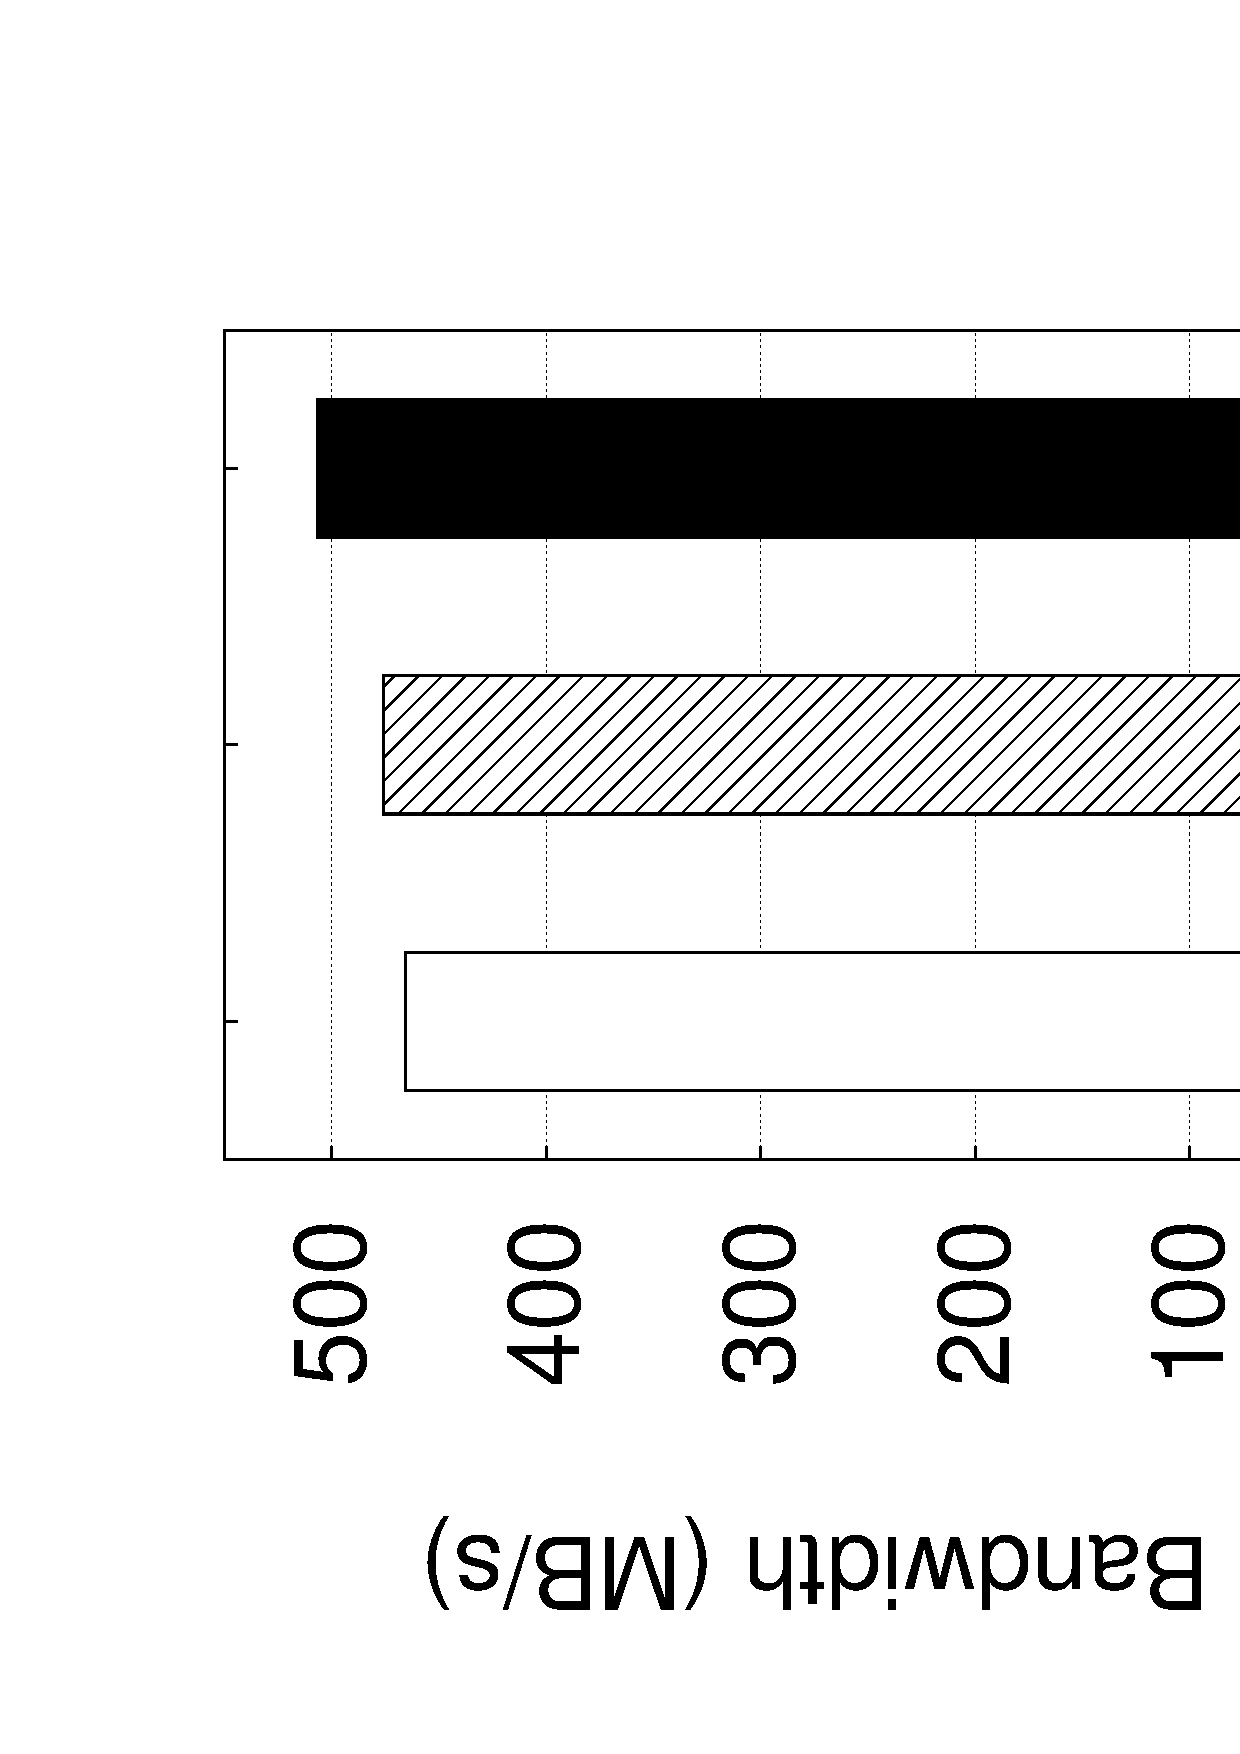
\includegraphics[angle=-90,width=1.55in]{./bench/seq_write}
 \label{fig:benchtest_seqw}
 }\hspace{-1.3em}
 \subfigure[Random Write]{
 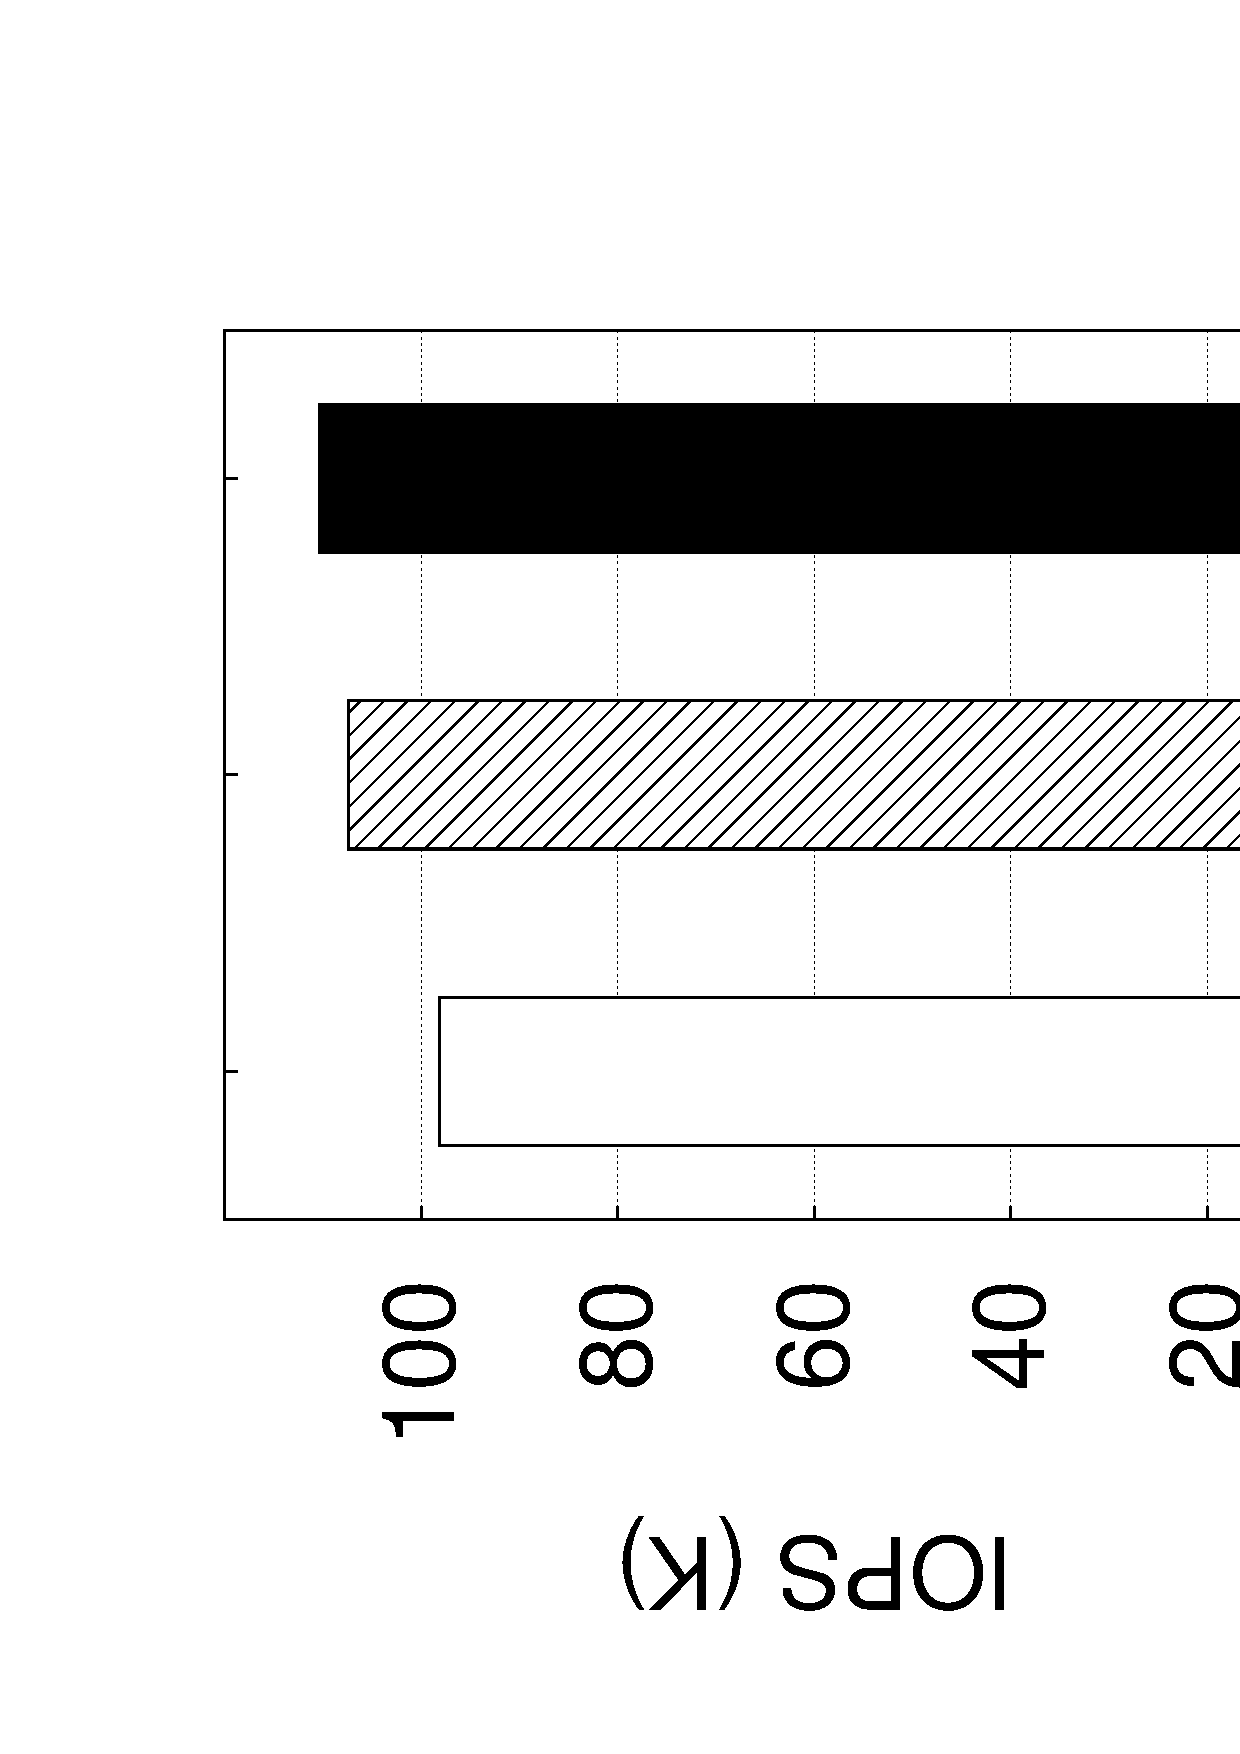
\includegraphics[angle=-90,width=1.55in]{./bench/rand_write}
 \label{fig:benchtest_randw}
 }
 \caption{Sequential / Random Write Performance, F2FS and Ext4 are on
   Page mapping SSD (Workload is as follows. Sequential Write: 188
   Gbyte File size, 512 Kbyte record size, 2.75 Tbyte Total write
   volume / Random Write: 50 Gbyte File size, 4 Kbyte record size, 750
   Gbyte Total write volume, Section size of F2FS: 256 Mbyte)}
 \vspace{-0.5em}
 \label{fig:benchtest}
\end{figure}

\begin{figure}[h]
  \begin{center}
  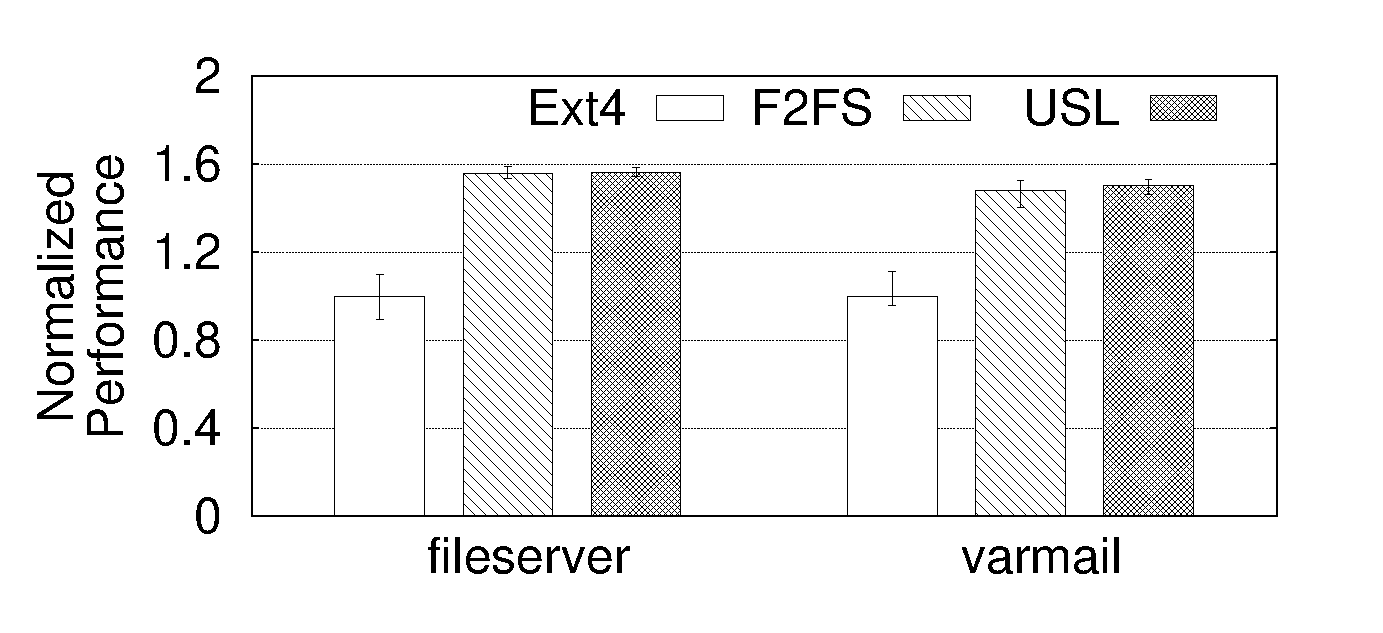
\includegraphics[width=3.2in]{./bench/filebench.eps}
  \vspace{-1em}
  \caption{Filebench Test Results}
  \vspace{-1.5em}
  \label{fig:filebench}
  \end{center}
\end{figure}

\subsection{IO Performance: Primitive IO}
\label{subsec:io_performance}

We measure the performance of different systems where neither garbage
collection nor segment cleaning occur. This is to examine the efficiency
of the code and the physical storage layout. Fig. \ref{fig:benchtest}
shows the performance of sequential write and random write. 


Ext4 and F2FS are mounted on page mapping SSD and USL uses
disaggregate mapping SSD with modified F2FS. Details of the environment is
described in Section \ref{subsec:exp_setup}. To measure the
sequential write performance, we format the file system and create a
file with size of 188 Gbyte. One iteration of an experiment issues 512
Kbyte buffered sequential write until all LBAs are covered and
repeat the iteration for fifteen times.
Fig. \ref{fig:benchtest_seqw} shows the average performance. The
performance of Ext4 and F2FS is 466 Mbyte/sec and 476 Mbyte/sec,
respectively. The performance of USL shows about 507
Mbyte/sec. It is 6$\%$ higher than that of F2FS.

The performance gap between Ext4 and USL stands out even
more in random write workload (Fig. \ref{fig:benchtest_randw}). 
To measure the random performance of
the device, we format the device and create a 50 Gbyte sized file in
the partition. An iteration of the experiment touches all the LBAs
with 4 Kbyte buffered random writes, and the graph shows the average of
fifteen iterations. The result shows that USL is about 12$\%$ faster
than Ext4; IOPS of USL is 110.3 KIOPS and Ext4 is 98.1 KIOPS. 

\begin{comment}
  \begin{figure}[t]
    \begin{center}
    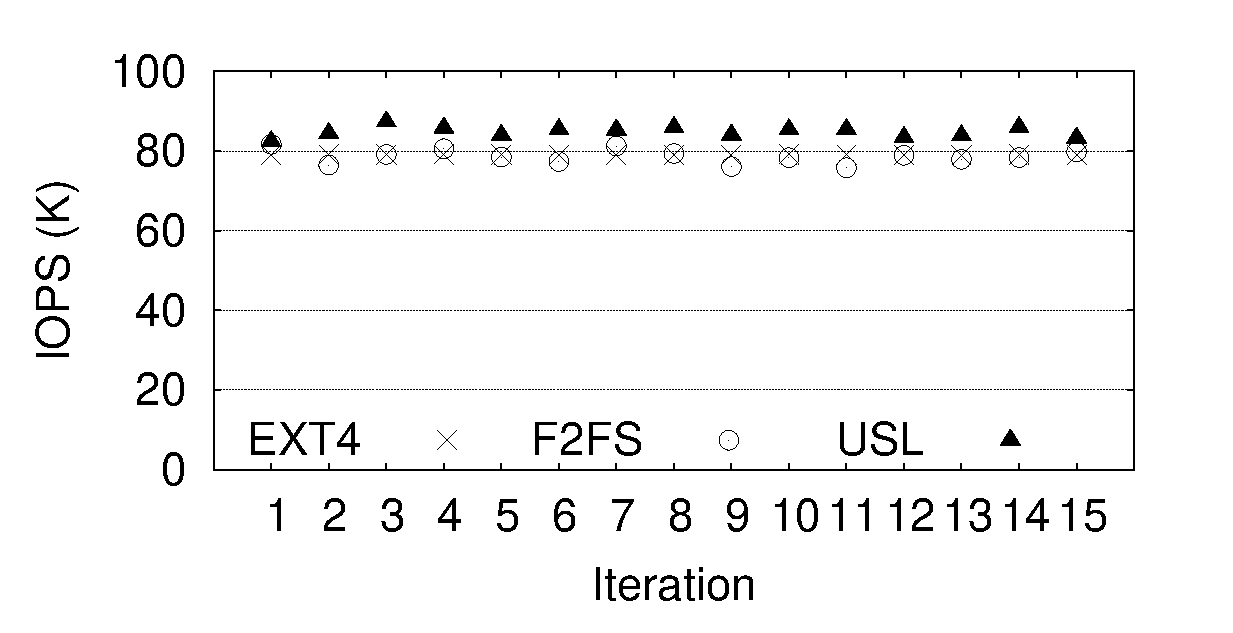
\includegraphics[width=3.3in]{./bench/mobibench_randw_iops.eps}
    \caption{Mobibench 4 Kbyte Random Write Test (170 Gbyte Cold data,
      20 Gbyte Hot data, Section size of F2FS: 256 Mbyte)}
    \label{fig:mobibench_randw}
    \vspace{-1.5em}
    \end{center}
  \end{figure}

  Fig \ref{fig:mobibench_randw} shows average IOPS of fifteen iterations of
  random write I/O generated by Mobibench benchmark tool
  \cite{jeong2013androstep}. After formatting the partition, we create
  a 170 Gbyte sized file as a cold data, and create another 20 Gbyte
  sized file as a hot data. An iteration of experiment writes 20 Gbyte
  file with 4 Kbyte buffered random write. This workload also shows no
  sign of garbage collection because free space available in the
  file system partition is larger than the hot data we used in the
  experiment. The result shows that IOPS of F2FS (80.5 KIOPS) and Ext4
  (81.0 KIOPS) is not much different from each other. On the other hand,
  USL is slightly faster than the other systems, it shows about 8$\%$
  higher random write IOPS (86.8 KIOPS).
\end{comment}

\subsection{Performance: Micro Benchmark}

Fig. \ref{fig:filebench} shows the result of filebench \cite{filebench} in
\emph{fileserver} and \emph{varmail} workload. The performance is
normalized with respect to the performance of Ext4. In the case of
fileserver workload, 
EXT4 shows 225 Mbyte/sec where F2FS and USL exhibits 350 Mbyte/sec and
352 Mbyte/sec, respectively. USL shows 1.6 times better performance
than Ext4. The result is similar in varmail. The performance of USL is
29 Mbyte/sec and Ext4 is 20 Mbyte/sec which is 1.5 times higher.
{\color{red} The performance difference comes from the size of the
blocks passed with \texttt{discard} command \cite{lee2015f2fs}.: yjwon:
good point!, by the way do we have evidence?}
Ext4 sends a lot of small sized discard commands but F2FS and USL sends
at least segment sized discard commands which significantly reduces the
overhead of processing discard commands in the device.  

\subsection{Effect of Eliminating the Compound Garbage Collection}
\label{subsec:remove_gc_overhead}

We measure the performance of USL and compare it with F2FS. 
The compound garbage collection is a problem only exists in stacked log 
system. And, to give a fair trial between the log-structured
filesystems, we only compare the result of F2FS and USL. Precondition
of experiments is as follows. We format the device and create a
partition using available 256 Gbyte of space; create 170 Gbyte
file. Single iteration of experiment generates total 85 Gbyte volume of
4 KByte random write on the created file. The ranges of the writes are
limited from 0 to 85 Gbyte LBAs of the file. We repeat the 
iteration fifteen times and measure the WAF and the performance of
each iteration. We used \texttt{smartmontools}
package\cite{smartmontools} to get the WAF of storage. 
The result shown at Fig. \ref{fig:f2fs_vs_usl} is
the average of fifteen iterations.




\begin{figure}[t]
  \centering
  \subfigure[WAF]{
    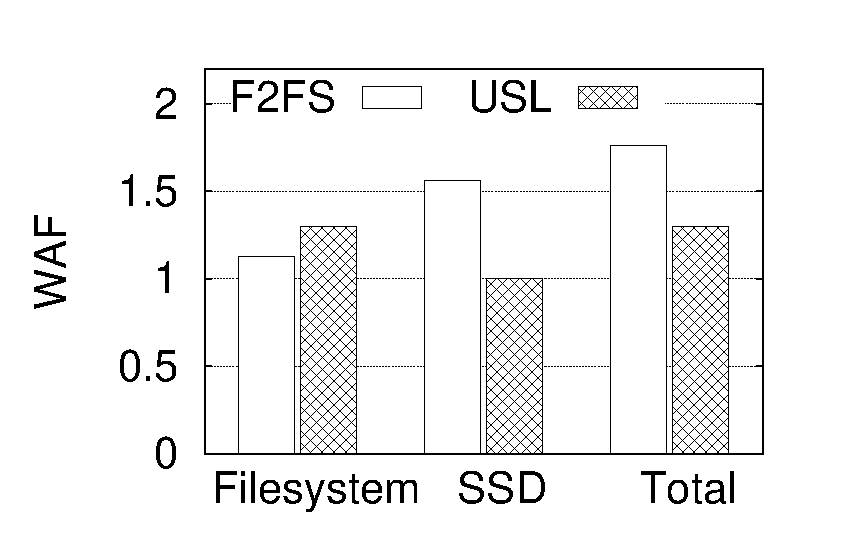
\includegraphics[width=2.1in]{./comp_gc/f2fs_vs_usl_waf}
   \label{fig:f2fs_vs_usl_waf}
   }
   \subfigure[IOPS]{
   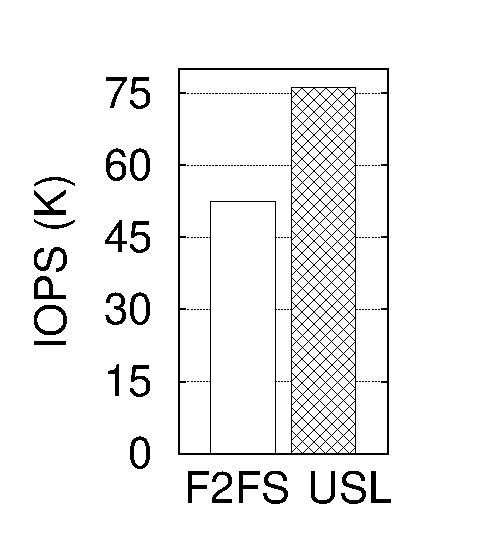
\includegraphics[width=1.1in]{./comp_gc/f2fs_vs_usl_iops}
   \label{fig:f2fs_vs_usl_iops}
   }
   \caption{WAF and IOPS of Each System
     (85 Gbyte Cold File, 85 Gbyte Hot File, 4 Kbyte buffered random write to the Hot File, 170 Gbyte Total write volume, Section size of F2FS: 256 Mbyte)\label{fig:f2fs_vs_usl}}
\vspace{-1.5em}
\end{figure}

\begin{comment}
\begin{figure*}[t]
\label{fig:170_85_randw}
\centering

\subfigure[File System WAF]{
 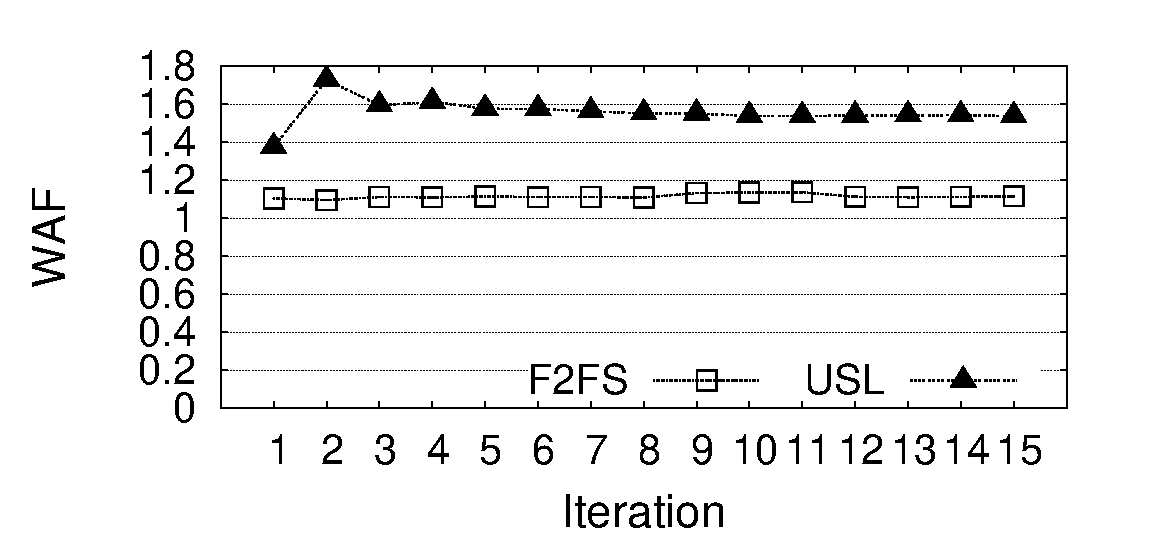
\includegraphics[width=3.3in]{./comp_gc/170_85_randw_fs}
 \label{fig:170_85_randw_fs}
 }
\subfigure[Device WAF]{
 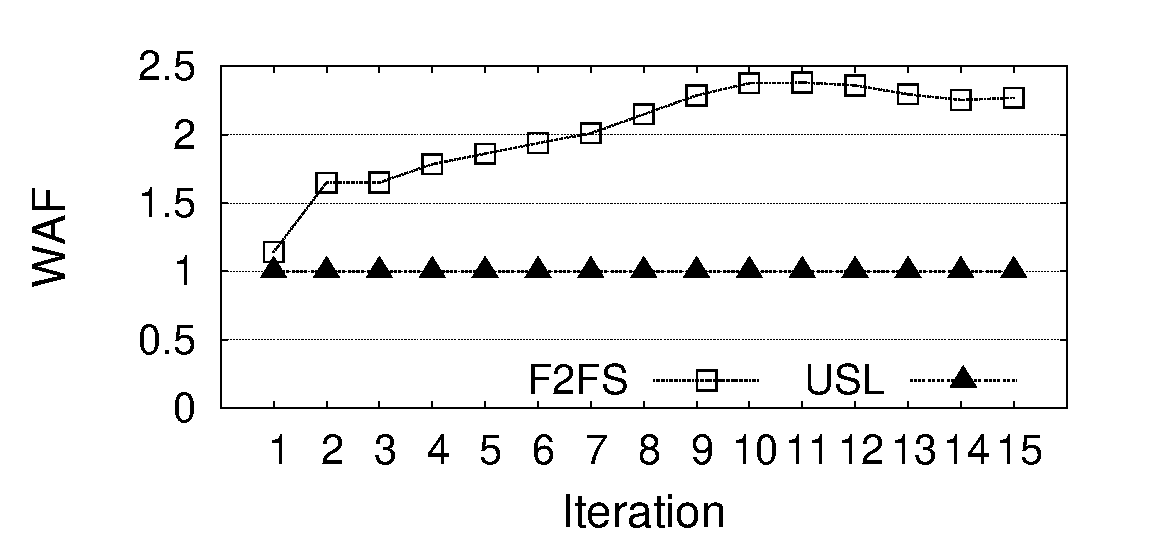
\includegraphics[width=3.3in]{./comp_gc/170_85_randw_dev}
 \label{fig:170_85_randw_dev}
 }
\subfigure[Total WAF]{
 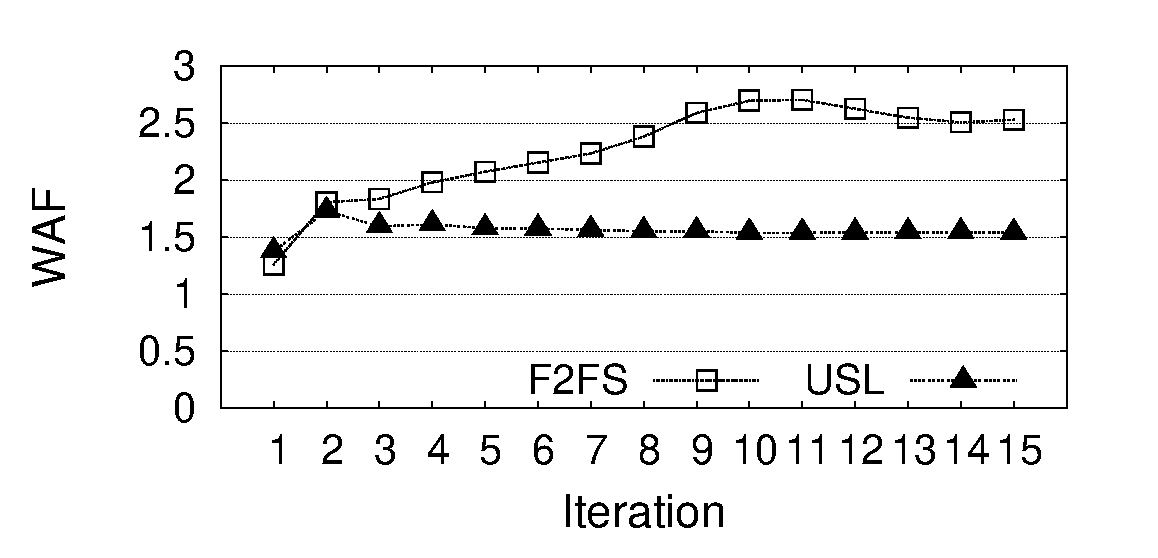
\includegraphics[width=3.3in]{./comp_gc/170_85_randw_total}
 \label{fig:170_85_randw_total}
 }
 \subfigure[IOPS]{
 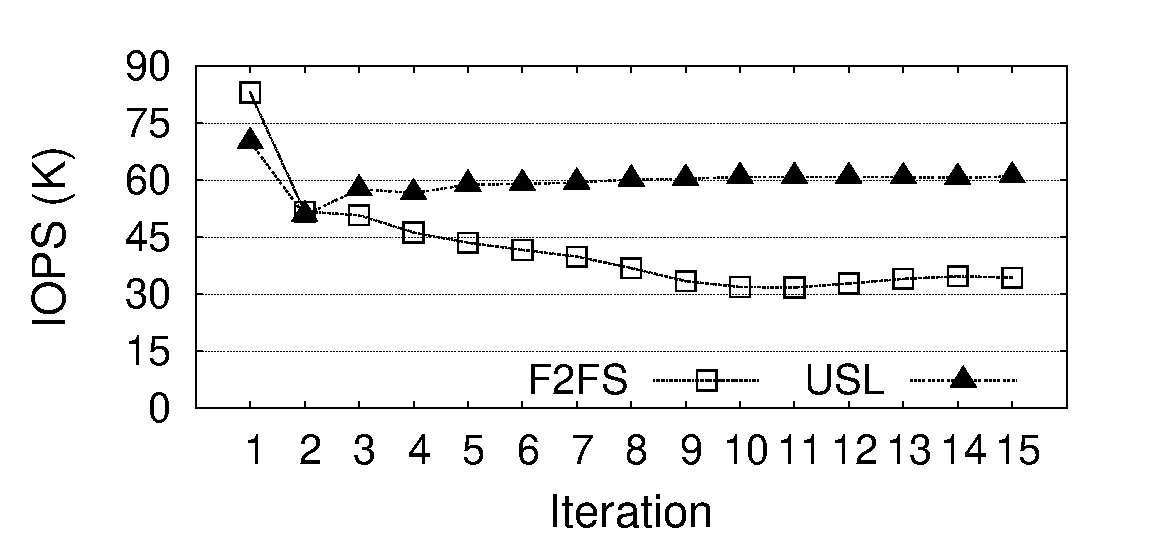
\includegraphics[width=3.3in]{./comp_gc/170_85_randw_iops}
 \label{fig:170_85_randw_iops}
 }
 \caption{The Result of Compound Garbage Collection in Case Study 2
   (Section size of F2FS: 256 Mbyte)\label{fig:170_85_randw}}
\end{figure*}
\end{comment}


Fig. \ref{fig:f2fs_vs_usl_waf} shows the WAF observed on the filesystem
and the device along with the total WAF. The result shows that using USL
increases filesystem WAF by 15\% compared to that of F2FS with page
mapping SSD. On the other hand, the WAF of device shows that USL is 36\%
better than existing F2FS. Overall, the total WAF of USL is 26\% lower
than that of F2FS. Fig. \ref{fig:f2fs_vs_usl_iops} shows IOPS of each
configuration. As a result of keeping the overall WAF low, USL achieved
about 45\% better IOPS than F2FS. 

Fig. \ref{fig:io_distribution} illustrates the write volume generated
for data update, metadata, filesystem segment cleaning, and device garbage
collection in writing 85 GByte of blocks. An iteration of random write
with F2FS generates total of 149 Gbyte of write requests to storage, but
USL generates only 113 Gbyte of write requests to storage, which is
about 24\% lower. 


Metadata write volume of USL is 613 Mbyte which is about 170 Mbyte
higher than that of F2FS. Although user requested to write 85 Gbyte of
data to the SSD, total volume written to the storage is about 150 Gbyte,
where about 11 Gbyte are generated by segment cleaning and about 53
Gbyte is generated by garbage collection.  The total volume written to
the storage in USL is about 24$\%$ lower than  that of Ext4 because USL
not only removes the effect of compound garbage collection but also
removes the random I/Os generated by threaded logging scheme.  






\begin{figure}[t]
\begin{center}
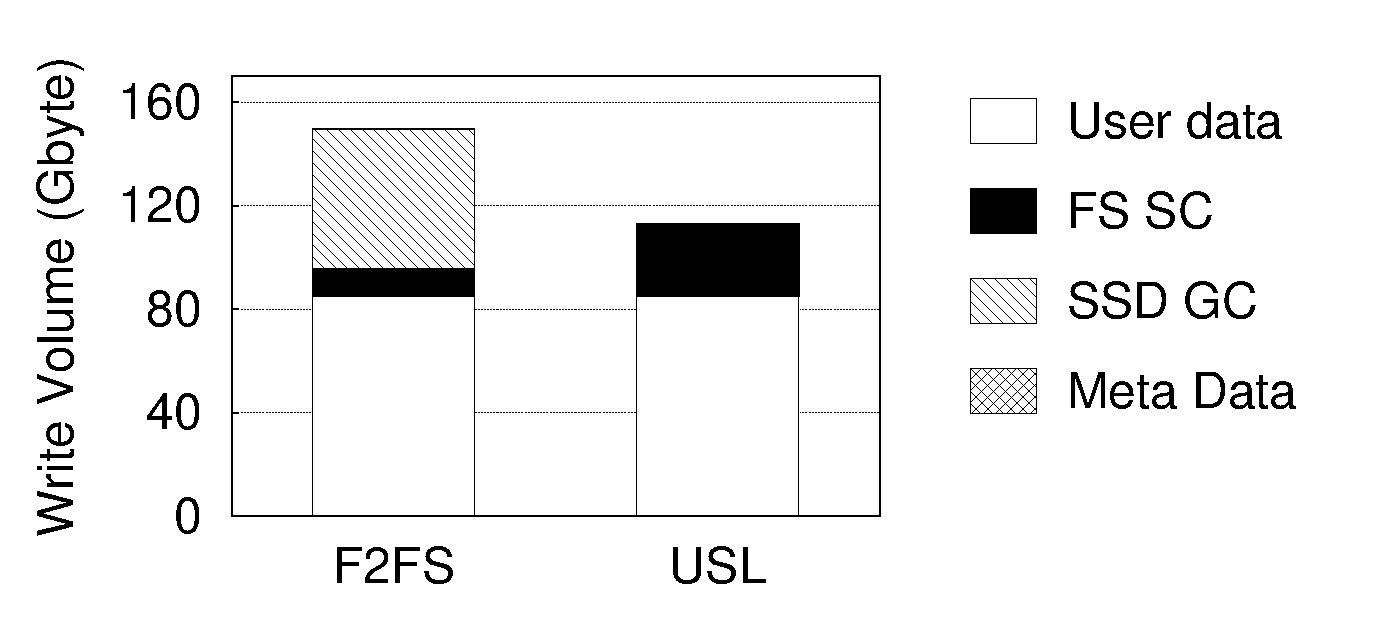
\includegraphics[width=3.2in]{./comp_gc/io_distribution.eps}
\caption{Total Write Volume Distribution (4 Kbyte buffered random write, Write volume generated by the application is 85 Gbyte, Section size of F2FS: 256 Mbyte)}
\label{fig:io_distribution}
\vspace{-1.5em}
\end{center}
\end{figure}


\begin{figure}[t]
\begin{center}
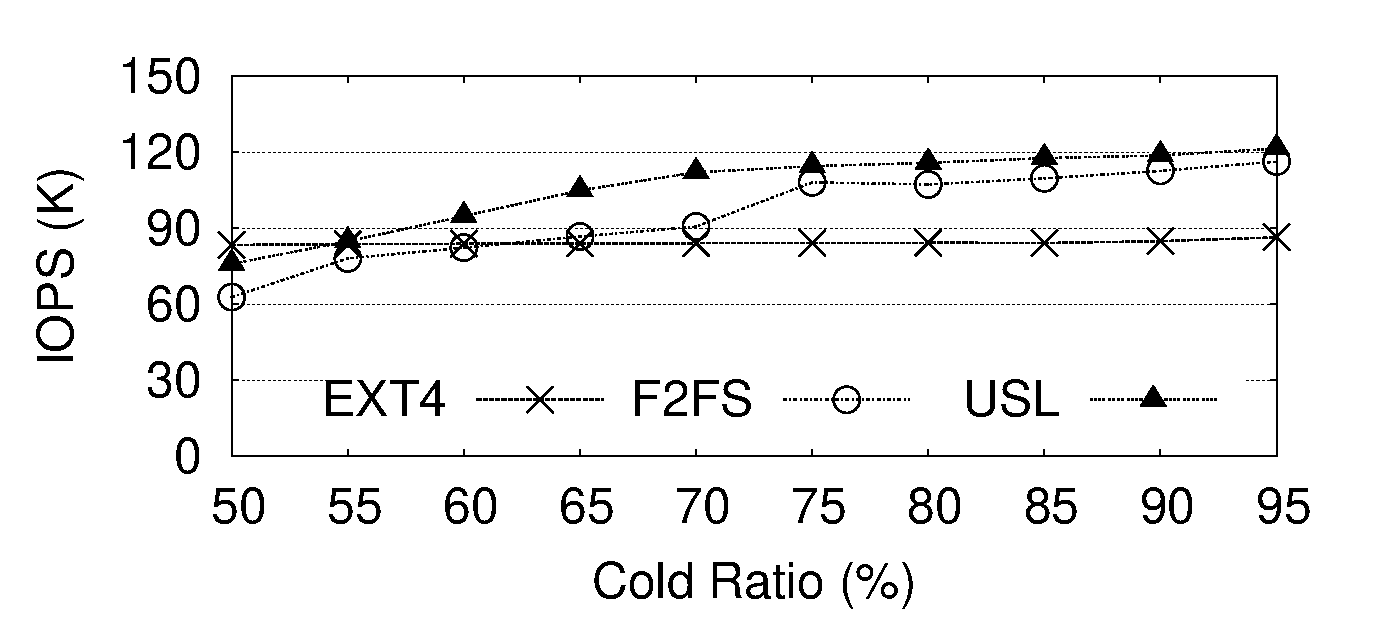
\includegraphics[width=3.2in]{./comp_gc/cold_ratio_iops.eps}
\caption{Random Write Performance according to the Cold Data Ratio (The total size of cold data and hot data is 170 Gbyte, Section size of F2FS: 256 Mbyte)}
\label{fig:cold_ratio_iops}
\vspace{-1.5em}
\end{center}
\end{figure}

\begin{figure}[t]
\begin{center}
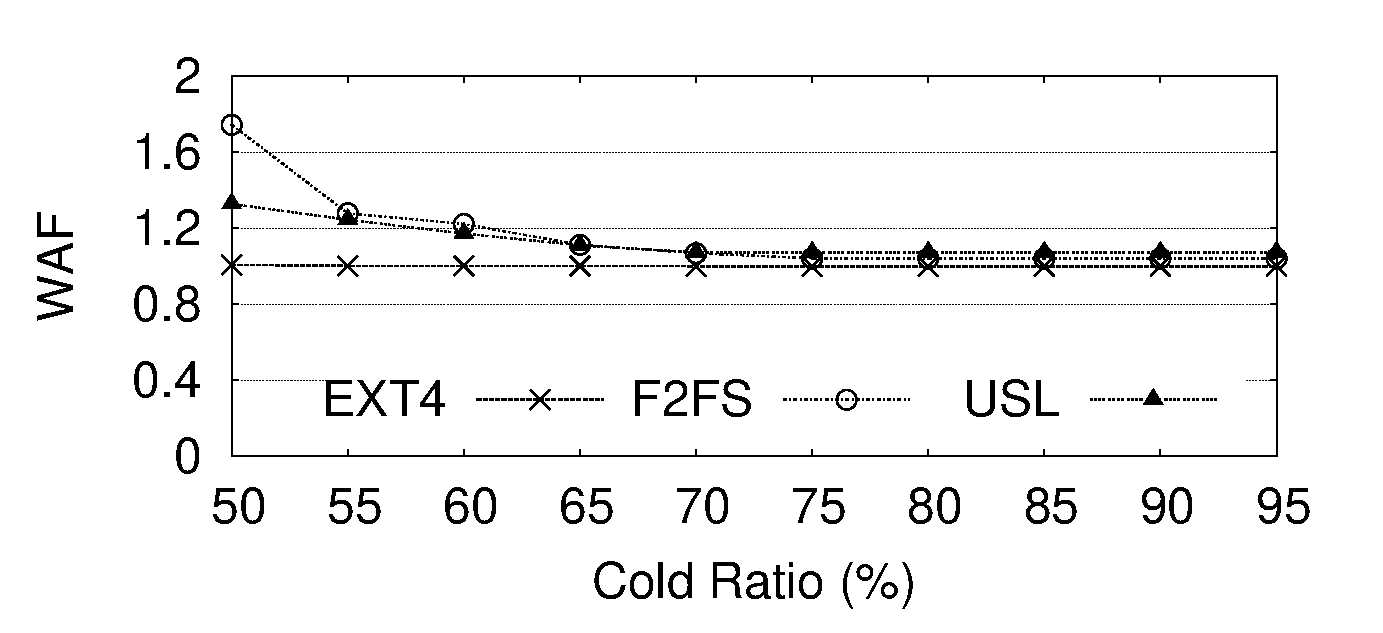
\includegraphics[width=3.2in]{./comp_gc/cold_ratio_waf.eps}
\caption{WAF according to the Cold Data Ratio (The total size of cold data and hot data is 170 Gbyte, Section size of F2FS: 256 Mbyte)}
\label{fig:cold_ratio_waf}
\vspace{-1.5em}
\end{center}
\end{figure}


\subsection{Cold block ratio and Segment Cleaning Overhead}
\label{section:cbr}
In most storage devices, the dominant fraction of the storage is filled
with cold files which are barely updated or accessed \cite{park2011hot}. We
examine the performance of different storage stacks varying the fraction
of cold data over entire storage partition.

Fig. \ref{fig:cold_ratio_iops} shows the result of 4 Kbyte buffered
random writes to hot file on three file systems while varying the size of cold data. 
The relationship between hot file size ($F_{hot}$), cold file size ($F_{cold}$), 
and the total volume ($TotalVolume$) in Gbytes used in the experiment is as follows: 
$F_{cold} + F_{hot} = TotalVolume$ and $TotalVolume \times ( 1 - x ) = F_{hot}$.
We set $TotalVolume = 170$ and $x$ equals to ratio of $TotalVolume$, 
which we vary from 50$\%$ to 95$\%$. For example, when $TotalVolume = 170$ 
and $x = 0.6$, the size of hot data is $170 \times 0.4 = 68$ Gbyte and 
the cold data is 102 Gbyte. We repeat the experiment fifteen times, and the total
volume written in an iteration is 170 Gbyte. The result shows the average of fifteen iterations. 

In all cases, USL outperforms the result of F2FS; USL is about 21$\%$
faster than F2FS when the cold ratio is 50$\%$ and the difference
closes into 4$\%$ when the cold ratio becomes 95$\%$. It shows that the
effect of compound garbage collection becomes less significant as the
hot ratio becomes smaller. The performance of Ext4 is stable around 83.5 $\sim$ 86.5
KIOPS. The performance of USL becomes higher than Ext4 when the cold
ratio is less than 55$\%$ and the gap widens as the ratio
decreases. When the cold ratio set to 95$\%$, USL shows about 41$\%$
higher IOPS than that of Ext4. Considering the report that the size
of the hot data in the system is about 5 to 25$\%$ of the workload
\cite{park2011hot}, it is reasonable to say that the
performance of USL is superior to other systems, especially when most
of the partition is filled with cold data and only small amount of
data is frequently accessed. 

Fig. \ref{fig:cold_ratio_waf} shows $WAF^{sys}$ of the result in 
Fig. \ref{fig:cold_ratio_iops}. Overall, the result shows that 
$WAF^{sys}_{f2fs}$ is higher than $WAF^{sys}_{usl}$. As it is described in
Section \ref{subsec:remove_gc_overhead}, F2FS has higher WAF than other systems
because of the write amplification caused by compound garbage collection.
It has to be noted that although $WAF^{sys}_{ext4}$ is the lowest, but IOPS on
USL is higher than that of Ext4. It is because all random writes in USL are
sequentially logged to the storage.


The proposed USL with disaggregate mapping allows not only reducing the
device level garbage collection but also lowering the total WAF of the
system.

\begin{figure}[t]
\begin{center}
\includegraphics[width=1.5in, angle=-90]{./comp_gc/segs_per_sec.eps}
\caption{4 Kbyte Buffered Random Write Performance according to the Section size}
\label{fig:segs_per_sec}
\vspace{-1.5em}
\end{center}
\end{figure}

\subsection{Effect of Segment Cleaning Unit}

Increase in WAF for compound garbage collection means one thing:
misalignment of garbage collection unit between storage and
file system. To illustrate the effect of misalignment,
Fig. \ref{fig:segs_per_sec} shows the performance of F2FS and USL while
varying the size of a section, which is the unit of segment cleaning in
F2FS. For comparison, we used same condition and workload used in
Fig. \ref{fig:f2fs_vs_usl}. The size of the section is increased from 2
Mbyte to 256 Mbyte in multiples of two. X-axis of the graph shows the
size of a section and used in the file system. Y1-axis and Y2-axis show IOPS and
WAF of experiments, respectively. The result shows that as section
size increases the performance also increases, and the
performance is the highest when the size of the section matches 
the garbage collection unit of the storage device. 
Compared to the IOPS and WAF of F2FS with section size of 2 Mbyte,
F2FS with section size 256 Mbyte shows 24$\%$ higher IOPS and 20$\%$ lower WAF.

It is important to match the garbage collection unit between filesystem
and storage device to reduce the garbage collection overhead in stacked
log system. Even though the section size of F2FS is matched with the
garbage collection unit of SSD, the effect of compound garbage
collection is not completely removed. As a result, the performance of
USL is about 24$\%$ higher than F2FS with 256 Mbyte section size.  




\begin{comment}
  \subsection{Multi-threaded Write}

  Fig. \ref{fig:50_50_seqw_waf} shows the Total WAF---file system WAF
  $\times$ device WAF---of F2FS and USL while processing multi-threaded
  sequential update workload, which is described in Section
  \ref{subsec:case_study_3}. After formatting the partition, we create
  fifty 3.8 Gbyte files sequentially. Then, create fifty threads to
  write 0 to 1 Gbyte range of each file with 256 Kbyte buffered
  sequential update operation, which is one iteration of the experiment.

  Fig. \ref{fig:50_50_seqw_waf} shows the WAF of seven runs. Except the
  first iteration, USL shows about 15$\%$ lower WAF compared to the
  system with base F2FS. It shows that WAF of F2FS is in between 1.5 to
  2. As we have discussed in Section \ref{subsec:case_study_3}, although
  each thread issues sequential write requests, the group behavior of
  multi-threaded I/O requests may increase the overal WAF of the
  system. In the case of USL, file system triggers number of segment
  cleaning jobs, but since there is no device level garbage collection,
  USL shows WAF of 1.3 to 1.4, overall USL shows about 26$\%$ lower WAF
  than that of F2FS. 

  In this section, we observed that stacking log-structured system
  suffers from compound garbage collection, and it also showed that
  without proper coordination between the two systems, stacking log
  system is bounded to have high write amplification. Unified Storage
  Layer is combination of efforts to reduce the size of mapping table
  using disaggregate mapping and resolve compound garbage collection by
  delegating SSD level garbage collection to file system. And experiments
  in this section show that it successfully addresses the problem.
\end{comment}

\begin{comment}
  match the garbage collection unit between
  file system and storage device to resolve compound garbage
  collection. And experiments in this section shows that it successfully
  address the problem.
\end{comment}

\begin{comment}
  \begin{figure}[t]
  \begin{center}
  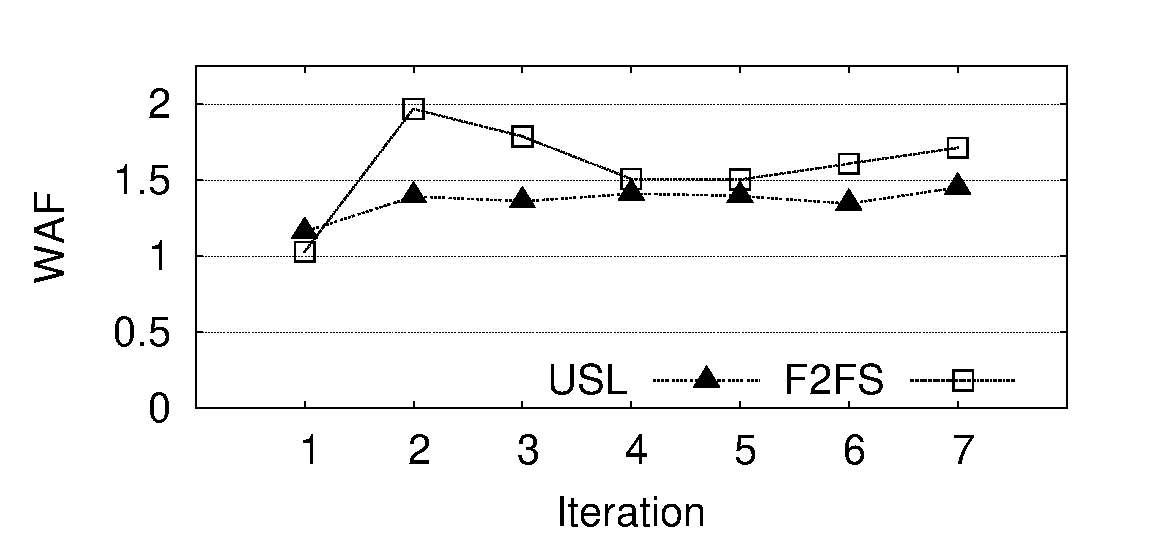
\includegraphics[width=3.5in]{./comp_gc/50_50_seqw_total}
  \caption{The Result of Compound Garbage Collection Scenario 3 (Section
    size of F2FS: 256 Mbyte)}
  \label{fig:50_50_seqw_waf}
  \vspace{-1.5em}
  \end{center}
  \end{figure}
\end{comment}

\section{Related Works}
\label{sec:related_works}

Lots of the efforts were focused on reducing the size of the mapping table 
or FTL. Many have tried to replace de facto FTL, that is page mapping FTL 
\cite{ban1995flash}, with various hybrid FTLs \cite{kang2006superblock,
fast07, last08}.  

Recent works tried to remove the level of indirection in SSD. There are
few different ways to remove the level of indirection  in the I/O stack.  
One of the ways is to introduce new I/O interface to the system. Zhang 
et al. \cite{zhang2012indirection} introduced nameless writes, a new
device interface to remove the mapping layer in FTL and opened its
physical addresses to the  filesystem. Saxena et
al. \cite{saxena2013getting} implemented 
nameless writes using OpenSSD Jasmin board. They found that directly accessing 
the physical address needs caution because programming to the Flash memory 
always have to follow its erase before update property. The characteristics 
becomes an issue especially when the write unit of the filesystem is different 
from that of SSD. NVMKV \cite{nvmkv}, on the other hand, replaces the operation for 
key-value operations with FTL commands, i.e., atomic multiple-block write, 
p-trim, exists, and iterate. Since the operations are substituted with FTL 
commands, the host is exempted from managing in-memory metadata for key-value 
store. NVMKV successfully removes the overhead of duplicate management of 
metadata and also reduces write amplification. Aforementioned works
successfully  reduce the level of indirection by introducing specific
interfaces or directly  using the FTL commands, however they are short
in solving problem of garbage  collection entirely.

Second category of the solution makes use of virtualized block device 
\cite{josephson2010dfs, lee2012ressd, kim2012advil, anvil, sdf, tuch2012block}
and Object-based SSDs \cite{lee2013ossd, lu2013extending}, 
which strives to minimize the overhead of stacked indirection layers and
garbage  
collection. They use a single mapping layer on the device or host to map files 
or objects to the pages containing their data. 

Direct File System, DFS \cite{josephson2010dfs} uses a virtualized block
device layer to improve the performance. DFS replaces the role of block
management and FTL through a layer called virtualized flash storage
layer (VFSL). The design of DFS is greatly simplified because VFSL
manages block allocation and inode management that used  to be
manipulated in filesystem. Logging Block Store \cite{tuch2012block} resolve a  
mismatch between the virtual memories I/O mixture and properties of block 
device in mobile devices. ReSSD \cite{lee2012ressd} and ADVIL \cite{kim2012advil}, which 
are virtual block device on top of an SSD, try to improve the small random 
write performance by transforming the requests to sequential writes. Both 
schemes \cite{lee2012ressd, kim2012advil} makes use of reserved area to stage the incoming random 
writes. Their approaches are more or less similar to log-structured system 
that suffers from the overhead of garbage collection. 

In order to reduce the level of indirection ANViL \cite{anvil} and FSDV \cite{zhangremoving} provides 
a way for the host to access the physical address mapping information. ANViL 
\cite{anvil} lets the host to modify device logical-to-physical mapping information 
through a new I/O interfaces. Host exploits the given interfaces to remove 
redundant data copy overhead and provide useful features such as single 
journaling and file snapshot to the system. FSDV (File Ssytem De-Virtualizer) 
\cite{zhangremoving} is a user-lvel tool that reduces the memory overhead of managing mapping 
information on both filesystem and storage device. When FSDV is invoked, it 
first checks mapping information and makes filesystem to point the physical 
address and removes logical to physical address mapping information on SSD 
mapping table. One of the downside of using FSDV is that the memory on the 
device cannot be smaller than the maximum size of the mapping table. 

Object-based SSDs \cite{lee2013ossd, lu2013extending} tries to overcome the limitations 
of the traditional block-level interface by virtualizing the physical storage 
into a pool of objects. OSSD \cite{lee2013ossd} implemented object-based SSD to 
simplify the host file system, utilize block-level liveness information to 
optimize on-disk layout, manage metadata, hot/cold data separation. OFSS 
\cite{lu2013extending} uses an object-based FTL with set of object
interfaces to compact and co-locate the small updates with
metadata. OFSS exploits backpointer to delay the persistence of the
object indexing. 

{\color{red}After analyzing the I/O patterns of in-house servers, Baidu 
introduced SDF (software-defined Flash) \cite{sdf}. The I/O patterns of their servers 
are mostly sequential and does not exhibit temporal locality. They made two 
interesting design choices. First, each Flash channel in SDF is considered as 
a separate storage device to host processes. Second, host is able to send Flash 
erase command which then allowed removing the overprovisioning area in the storage.}

Baidu introduced SDF (Software-defined Flash) to fully deliver the raw 
capacity of Flash memories and its bandwidth \cite{sdf}. SDF exposes
each Flash channels to the host as seperate block devices. 
By assigning the block devices to applications, SDF can provide channel
parallelism. Each channel 
engine in SDF is supposed to implement mapping table management, bad block
management and wear-leveling. The host performs garbage collection of the
device. Thus, Flash memories do not need to hold overprovisioning space.

A work that have same point of view with this paper is the work done by Yang 
et al. \cite{yang2014don}. They showed that it is better to keep the
size of upper segment larger or equal to the size of lower segment and
perform upper layer garbage  collection before lower layer garbage
collection to yield better performance.  





\section{Conclusion}
\label{sec:conclusion}

In this paper, we proposed Unified Storage Layer (USL) to solve two
problems: size of the mapping table of an SSD and compound garbage collection
of stacked log-structured systems. The mapping table in USL is managed
with disaggregate mapping which maintains two areas for different
purposes. Metadata area which is managed by page mapping is used for
metadata area of file system, and main area for user data is stored in
no mapping zone of the storage. Instead of keeping a mapping table for
main area, disaggregate mapping directly maps LBAs of the file system to
PBAs of the storage device. The use of disaggregate mapping reduced the
overall metadata size of an SSD to 1/54 compared to the de facto page
mapping scheme. Moreover, the static binding entirely eliminates the
root cause of compound garbage collection since the segment cleaning
of the log-structured file system directly consolidates the valid pages
in the Flash storage. WAF of USL is reduced by 26$\%$ and IOPS
increased about 45$\%$ against F2FS with an SSD. We believe that USL
not only minimizes the DRAM requirement for large scale SSDs but also
solves compound garbage collection in stacked log-structured system,
and it successfully increases the performance and life time of the
storage.

\bibliographystyle{IEEEtran}
%\bibliographystyle{acm}
\bibliography{ref}

%\pagebreak
%\tableofcontents


\begin{comment}
\subsection{Garbage Collection based Segment Cleaning}
\label{subsec:gc_based_sc}

Because the file system layer of USL is in charge of garbage 
collection for the main area, segment cleaning 
decides which NAND block should be erased. After the file system 
selects victim sections and performs segment cleaning on that sections, 
the file system sends 
the section numbers to the device. Upon receiving section numbers from the
file system, the storage device just erases the blocks in the sections.

When USL file system completes segment cleaning, it does not put
reclaimed section to free section; instead, it leaves the section as
pre-free section which only holds invalidated data. All pre-free
sections are put into free sections on file system checkpoint, and the
new free section numbers are delivered to the device. Upon receiving
the free section numbers, the device erases the corresponding NAND
blocks. Then the file system puts the section into a free section to serve incoming I/O
requests.

USL requires means to transfer the acquired set of section
numbers from file system segment cleaning process to the storage
device. We used SATA write command to send section numbers.
To distinguish ordinary write calls from sending section numbers, 
we used SATA command extension. The payload of the command has
new free section numbers.
When the SSD receives the SATA command extension, the firmware of the SSD recognizes
the write call as information about the section numbers to erase. Upon receiving 
section numbers from the file system via write system call, the storage 
device needs to just erase the blocks. 

\begin{comment}
  Since all PBAs are matched to LBAs of main area of USL
  file system, the storage device does not perform garbage collection on
  those blocks; instead, the file system performs segment cleaning and
  sends the section numbers that needs to be erased from the storage.
\end{comment}


\section{Analytical Analysis}
\label{sec:measuring_waf}

The performance of a file system or a storage system can be represented
with a notion called Write Amplification Factor, WAF
\cite{rosenblum1992design}, which is defined as a ratio of the amount
of write volume received from a higher level I/O layer and the actual
amount of write volume the lower level I/O layer has to process. 
In general, higher the WAF means
lower the performance because of the volume it has to process. In a
stacked log system, the combination of segment cleaning and garbage
collection on different layers leads to higher WAF.

In this section, we provide analytical WAF of Ext4 ($WAF_{ext4}$), F2FS
($WAF_{f2fs}$), and USL ($WAF_{usl}$) to have a better understanding of
the overhead. There are three factors that increase the WAF, they are
metadata, journal data, and segment cleaning. We use $W_{meta}$,
$W_{journal}$, and $W_{sc}$ to denote the total volume of blocks the
file system updates metadata, writes journal logs to journal area, and
processes to segment cleaning, respectively.

Although Ext4 is
in-place update file system which does not perform garbage collection,
write I/Os can be amplified through logging journal data. Thus, when a
user requests a write I/O with size $W_{data}$, the WAF of Ext4 can be
described as Eq. (\ref{eq:waf_ext4}).

\begin{equation}
\label{eq:waf_ext4}
WAF_{ext4} = \frac{W_{data}+W_{meta}+W_{journal}}{W_{data}+W_{meta}}\nonumber
\end{equation}
\vspace{-0.5em}
\begin{equation}
= 1+\frac{W_{journal}}{W_{data}+W_{meta}}
\end{equation}


If $W_{journal} \ll \left( W_{data} + W_{meta} \right) $ is true,
then we can say $WAF_{ext4} \approx 1$, but when $W_{journal} \approx
\left( W_{data} + W_{meta} \right)$, the WAF of Ext4 becomes close to 2.  
On the other hand, since F2FS and USL
perform segment cleaning, $WAF_{f2fs}$ and $WAF_{usl}$ can be
described as Eq. (\ref{eq:waf_f2fs}).


\vspace{-0.5em}
\begin{equation}
\label{eq:waf_f2fs}
WAF_{lfs} = \frac{W_{data}+W_{meta}+W_{sc}}{W_{data}+W_{meta}}\nonumber
\end{equation}
\vspace{-0.5em}
\begin{equation}
= 1+\frac{W_{sc}}{W_{data}+W_{meta}}
\end{equation}


WAF of the overall system with SSD, denoted as $WAF^{sys}$, is equal to
WAF of file systems multiplied by WAF of SSD, $WAF_{SSD}$. Then, WAF of
the overall system with Ext4 and F2FS can be described as
Eq. (\ref{eq:waf_sys_ext4}) and Eq. (\ref{eq:waf_sys_F2FS}),
respectively. We assume that $W_{journal}$ is very small and thus,
$WAF_{ext4}$ is also very small. 

\begin{equation}
\label{eq:waf_sys_ext4}
WAF^{sys}_{ext4} = WAF_{ext4}\times WAF_{ssd} \approx  WAF_{ssd}
\end{equation}
\vspace{-1em}
\begin{equation}
\label{eq:waf_sys_F2FS}
WAF^{sys}_{f2fs} =(1+\frac{W_{sc}}{W_{data}+W_{meta}})\times WAF_{ssd}
\end{equation}


Eq. (\ref{eq:waf_sys_ext4}) and Eq. (\ref{eq:waf_sys_F2FS}) show that
$WAF^{sys}$ is generally bounded by $WAF_{ssd}$ and takes segment
cleaning overhead of the file system as the coefficient. From the equation,
it becomes clear that $WAF_{f2fs}$ is generally larger when the
file system is performing segment cleaning. On the other hand, when the
system utilizes USL, $W_{ssd}$ is much smaller than that of F2FS
because USL uses segment cleaning only to small metadata area. As a
result, $WAF_{ssd}$ becomes approximately equal to 1, and we get
Eq. (\ref{eq:waf_sys_usl}). 


\vspace{-0.5em}
\begin{equation}
\label{eq:waf_sys_usl}
WAF^{sys}_{usl} = WAF_{usl}\times WAF_{ssd} \approx WAF_{usl}
\end{equation}


Note that $WAF_{usl}$ is only affected by $W_{sc}$, which implies that
it does not suffer from the overhead of compound garbage collection as
$WAF_{f2fs}$. 


\begin{comment}
  We provide analytical WAF of an in-place update file system, Ext4, and
  a log-structured file system, F2FS, to compare the inherent performance
  differences between the two file systems. 
  WAF를 증가시키는 요인으로는 메타데이터 관련 입출력, 저널링 동작, 그리고
  가비지 컬렉션 등이 있다. We assumed that metadata and journaling
  related I/O volume is significantly lower than that of user data and
  garbage collection related I/O volume and excluded from the computation.
  Overall system WAF is denoted as $WAF_{Total}$, file system WAF as $WAF_{fs}$, 
  and storage device level WAF as $WAF_{SSD}$.

  Analytical file system WAF of Ext4 is 1 because it is an in-place
  update file system. In a storage system with Ext4, the performance
  bottleneck would be garbage collection of the storage device. Thus,
  total WAF of Ext4 system can be represented as Eq. (\ref{eq:waf_ext4}).

  \vspace{-0.5em}
  \begin{equation}
  \label{eq:waf_ext4}
  WAF_{Total}^{Ext4} = WAF_{SSD}
  \end{equation}

  Since segment cleaning on a log file system is a must, potentially a
  stacking log system suffers from garbage collection of invalid data on
  all log layers. Thus, the WAF of stacking log system with F2FS can be
  represented as Eq. (\ref{eq:waf_lls}).

  \vspace{-0.5em}
  \begin{equation}
  \label{eq:waf_lls}
  WAF_{Total}^{F2FS} = WAF_{fs}\times WAF_{SSD}
  \end{equation}

  Finally, total WAF of Unified Storage Layer (USL) is bounded by
  file system because it dispenses the need of garbage collection in
  storage device. Instead, USL only performs segment cleaning on
  file system and delivers list of sections to erase to the
  storage. Total WAF of USL can be represented as Eq. (\ref{eq:waf_usl}).

  \vspace{-0.5em}
  \begin{equation}
  \label{eq:waf_usl}
  WAF_{Total}^{USL} = WAF_{fs}
  \end{equation}

  Eq. (\ref{eq:waf_usl}) implies that 
  USL do not suffer from the overhead of compound garbage collection. 
  Additional benefit of using USL is that SSD does not need to maintain 
  a mapping table for main area, which significantly reduced the size 
  of mapping table.

  Since stacking log system with F2FS runs garbage collection on both
  layers, the system is mostly likely be sensitive to garbage collection
  behavior on each layer and naturally will have higher WAF than
  in-place update file systems. On the contrary, total WAF of Ext4 only
  depends on garbage collection performance of storage device. However,
  underlying SSD must use page mapping for performance reasons, but the
  fact that there is high cost in using it should not be taken lightly,
  especially when the capacity of device is increasing. In Section
  \ref{sec:CompoundGC}, we measure the effect of processing garbage
  collection on each layers of log system and WAF of different systems.
\end{comment}

\begin{comment}
\begin{equation}
\label{eq:waf_ext4}
WAF_{ext4} = \frac{W_{data}+W_{meta}+W_{journal}}{W_{data}+W_{meta}}\nonumber
\end{equation}
\vspace{-0.5em}
\begin{equation}
= 1+\frac{W_{journal}}{W_{data}+W_{meta}}
\end{equation}


If $W_{journal} \ll \left( W_{data} + W_{meta} \right) $ is true,
then we can say $WAF_{ext4} \approx 1$, but when $W_{journal} \approx
\left( W_{data} + W_{meta} \right)$, the WAF of Ext4 becomes close to 2.  
On the other hand, since F2FS and USL
performs segment cleaning, $WAF_{f2fs}$ and $WAF_{usl}$ can be
described as Eq. (\ref{eq:waf_f2fs}).


\vspace{-0.5em}
\begin{equation}
\label{eq:waf_f2fs}
WAF_{lfs} = \frac{W_{data}+W_{meta}+W_{sc}}{W_{data}+W_{meta}}\nonumber
\end{equation}
\vspace{-1em}
\begin{equation}
= 1+\frac{W_{sc}}{W_{data}+W_{meta}}
\end{equation}


WAF of overall system with SSD, denoted as $WAF^{sys}$, is equal to
WAF of file systems multiplied by WAF of SSD, $WAF_{SSD}$. Then, WAF of
overall system with Ext4 and F2FS can be described as
Eq. (\ref{eq:waf_sys_ext4}) and Eq. (\ref{eq:waf_sys_F2FS}),
respectively. We assume that $W_{journal}$ is very small and thus,
$WAF_{ext4}$ is also very small. 

\begin{equation}
\label{eq:waf_sys_ext4}
WAF^{sys}_{ext4} = WAF_{ext4}\times WAF_{ssd} \approx  WAF_{ssd}
\end{equation}
\vspace{-1em}
\begin{equation}
\label{eq:waf_sys_F2FS}
WAF^{sys}_{f2fs} =(1+\frac{W_{sc}}{W_{data}+W_{meta}})\times WAF_{ssd}
\end{equation}


Eq. (\ref{eq:waf_sys_ext4}) and Eq. (\ref{eq:waf_sys_F2FS}) show that
$WAF^{sys}$ is generally bounded by $WAF_{ssd}$ and takes segment
cleaning overhead of the filesystem as coefficient. From the equation,
it becomes clear that $WAF_{f2fs}$ is generally larger when the
filesystem is performing segment cleaning. On the other hand, when the
system utilizes USL, $W_{ssd}$ is much smaller than that of F2FS
because USL uses segment cleaning only to small metadata area. As a
result $WAF_{ssd}$ becomes approximately equal to 1, and we get
Eq. (\ref{eq:waf_sys_usl}). 


\vspace{-0.5em}
\begin{equation}
\label{eq:waf_sys_usl}
WAF^{sys}_{usl} = WAF_{usl}\times WAF_{ssd} \approx WAF_{usl}
\end{equation}


Note that $WAF_{usl}$ is only affectd by $W_{sc}$, which implies that
it does not suffer from the overhead of compound garbage collection as
$WAF_{f2fs}$. 


\begin{comment}
  We provide analytical WAF of an in-place update filesystem, Ext4, and
  a log-structured filesystem, F2FS, to compare the inherent performance
  differences between the two filesystems. 
  WAF를 증가시키는 요인으로는 메타데이터 관련 입출력, 저널링 동작, 그리고
  가비지 컬렉션 등이 있다. We assumed that metadata and journaling
  related I/O volume is significantly lower than that of user data and
  garbage collection related I/O volume and excluded from the computation.
  Overall system WAF is denoted as $WAF_{Total}$, filesystem WAF as $WAF_{fs}$, 
  and storage device level WAF as $WAF_{SSD}$.

  Analytical filesystem WAF of Ext4 is 1 because it is an in-place
  update filesystem. In a storage system with Ext4, the performance
  bottleneck would be garbage collection of the storage device. Thus,
  total WAF of Ext4 system can be represented as Eq. (\ref{eq:waf_ext4}).

  \vspace{-0.5em}
  \begin{equation}
  \label{eq:waf_ext4}
  WAF_{Total}^{Ext4} = WAF_{SSD}
  \end{equation}

  Since segment cleaning on a log filesystem is a must, potentially a
  stacking log system suffers from garbage collection of invalid data on
  all log layers. Thus, the WAF of stacking log system with F2FS can be
  represented as Eq. (\ref{eq:waf_lls}).

  \vspace{-0.5em}
  \begin{equation}
  \label{eq:waf_lls}
  WAF_{Total}^{F2FS} = WAF_{fs}\times WAF_{SSD}
  \end{equation}

  Finally, total WAF of Unified Storage Layer (USL) is bounded by
  filesystem because it dispenses the need of garbage collection in
  storage device. Instead, USL only performs segment cleaning on
  filesystem and delivers list of sections to erase to the
  storage. Total WAF of USL can be represented as Eq. (\ref{eq:waf_usl}).

  \vspace{-0.5em}
  \begin{equation}
  \label{eq:waf_usl}
  WAF_{Total}^{USL} = WAF_{fs}
  \end{equation}

  Eq. (\ref{eq:waf_usl}) implies that 
  USL do not suffer from the overhead of compound garbage collection. 
  Additional benefit of using USL is that SSD does not need to maintain 
  a mapping table for main area, which significantly reduced the size 
  of mapping table.

  Since stacking log system with F2FS runs garbage collection on both
  layers, the system is mostly likely be sensitive to garbage collection
  behavior on each layer and naturally will have higher WAF than
  in-place update filesystems. On the contrary, total WAF of Ext4 only
  depends on garbage collection performance of storage device. However,
  underlying SSD must use page mapping for performance reasons, but the
  fact that there is high cost in using it should not be taken lightly,
  especially when the capacity of device is increasing. In Section
  \ref{sec:CompoundGC}, we measure the effect of processing garbage
  collection on each layers of log system and WAF of different systems.
\end{comment}

\begin{comment}
\begin{equation}
\label{eq:waf_ext4}
WAF_{ext4} = \frac{W_{data}+W_{meta}+W_{journal}}{W_{data}+W_{meta}}\nonumber
\end{equation}
\vspace{-0.5em}
\begin{equation}
= 1+\frac{W_{journal}}{W_{data}+W_{meta}}
\end{equation}


If $W_{journal} \ll \left( W_{data} + W_{meta} \right) $ is true,
then we can say $WAF_{ext4} \approx 1$, but when $W_{journal} \approx
\left( W_{data} + W_{meta} \right)$, the WAF of Ext4 becomes close to 2.  
On the other hand, since F2FS and USL
performs segment cleaning, $WAF_{f2fs}$ and $WAF_{usl}$ can be
described as Eq. (\ref{eq:waf_f2fs}).


\vspace{-0.5em}
\begin{equation}
\label{eq:waf_f2fs}
WAF_{lfs} = \frac{W_{data}+W_{meta}+W_{sc}}{W_{data}+W_{meta}}\nonumber
\end{equation}
\vspace{-1em}
\begin{equation}
= 1+\frac{W_{sc}}{W_{data}+W_{meta}}
\end{equation}


WAF of overall system with SSD, denoted as $WAF^{sys}$, is equal to
WAF of filesystems multiplied by WAF of SSD, $WAF_{SSD}$. Then, WAF of
overall system with Ext4 and F2FS can be described as
Eq. (\ref{eq:waf_sys_ext4}) and Eq. (\ref{eq:waf_sys_F2FS}),
respectively. Ext4의 system waf는 Eq. (\ref{eq:waf_ext4})에서
journal region에 발생한 블록 쓰기 양 ($W_{journal}$)이 충분히 작다는
가정을 사용하여 전개하였다.


\begin{equation}
\label{eq:waf_sys_ext4}
WAF^{sys}_{ext4} = WAF_{ext4}\times WAF_{ssd} \approx  WAF_{ssd}
\end{equation}
\vspace{-1em}
\begin{equation}
\label{eq:waf_sys_F2FS}
WAF^{sys}_{f2fs} =(1+\frac{W_{sc}}{W_{data}+W_{meta}})\times WAF_{ssd}
\end{equation}


Eq. (\ref{eq:waf_sys_ext4}) and Eq. (\ref{eq:waf_sys_F2FS}) show that
$WAF^{sys}$ is generally bounded by $WAF_{ssd}$ and takes segment
cleaning overhead of the file system as coefficient. From the equation,
it becomes clear that $WAF_{f2fs}$ is generally larger when the
file system is performing segment cleaning. On the other hand, when the
system utilizes USL, $W_{ssd}$ is much smaller than that of F2FS
because USL uses segment cleaning only to small metadata area. As a
result $WAF_{ssd}$ becomes approximately equal to 1, and we get
Eq. (\ref{eq:waf_sys_usl}). 


\vspace{-0.5em}
\begin{equation}
\label{eq:waf_sys_usl}
WAF^{sys}_{usl} = WAF_{usl}\times WAF_{ssd} \approx WAF_{usl}
\end{equation}


Note that $WAF_{usl}$ is only affectd by $W_{sc}$, which implies that
it does not suffer from the overhead of compound garbage collection as
$WAF_{f2fs}$. 


\begin{comment}
  We provide analytical WAF of an in-place update file system, Ext4, and
  a log-structured file system, F2FS, to compare the inherent performance
  differences between the two file systems. 
  WAF를 증가시키는 요인으로는 메타데이터 관련 입출력, 저널링 동작, 그리고
  가비지 컬렉션 등이 있다. We assumed that metadata and journaling
  related I/O volume is significantly lower than that of user data and
  garbage collection related I/O volume and excluded from the computation.
  Overall system WAF is denoted as $WAF_{Total}$, file system WAF as $WAF_{fs}$, 
  and storage device level WAF as $WAF_{SSD}$.

  Analytical file system WAF of Ext4 is 1 because it is an in-place
  update file system. In a storage system with Ext4, the performance
  bottleneck would be garbage collection of the storage device. Thus,
  total WAF of Ext4 system can be represented as Eq. (\ref{eq:waf_ext4}).

  \vspace{-0.5em}
  \begin{equation}
  \label{eq:waf_ext4}
  WAF_{Total}^{Ext4} = WAF_{SSD}
  \end{equation}

  Since segment cleaning on a log file system is a must, potentially a
  stacking log system suffers from garbage collection of invalid data on
  all log layers. Thus, the WAF of stacking log system with F2FS can be
  represented as Eq. (\ref{eq:waf_lls}).

  \vspace{-0.5em}
  \begin{equation}
  \label{eq:waf_lls}
  WAF_{Total}^{F2FS} = WAF_{fs}\times WAF_{SSD}
  \end{equation}

  Finally, total WAF of Unified Storage Layer (USL) is bounded by
  file system because it dispenses the need of garbage collection in
  storage device. Instead, USL only performs segment cleaning on
  file system and delivers list of sections to erase to the
  storage. Total WAF of USL can be represented as Eq. (\ref{eq:waf_usl}).

  \vspace{-0.5em}
  \begin{equation}
  \label{eq:waf_usl}
  WAF_{Total}^{USL} = WAF_{fs}
  \end{equation}

  Eq. (\ref{eq:waf_usl}) implies that 
  USL do not suffer from the overhead of compound garbage collection. 
  Additional benefit of using USL is that SSD does not need to maintain 
  a mapping table for main area, which significantly reduced the size 
  of mapping table.

  Since stacking log system with F2FS runs garbage collection on both
  layers, the system is mostly likely be sensitive to garbage collection
  behavior on each layer and naturally will have higher WAF than
  in-place update file systems. On the contrary, total WAF of Ext4 only
  depends on garbage collection performance of storage device. However,
  underlying SSD must use page mapping for performance reasons, but the
  fact that there is high cost in using it should not be taken lightly,
  especially when the capacity of device is increasing. In Section
  \ref{sec:CompoundGC}, we measure the effect of processing garbage
  collection on each layers of log system and WAF of different systems.
\end{comment}

\begin{comment}
\section{Write Amplification Analytic Model}
\label{sec:WA_model}


%5장의 존재 의미
Write amplification (WA) measures the the number of user page writes
against actual number of page writes. Since SSDs are out-of-place
update device, WA can describe the performance of the
device. Through modeling of WA of SSDs, we try to understand the
theoretical performance of the device and use it to analyze the
bottleneck in the system. 


%기존의 WAF analytic model
There are number of works in the field to provide analytical model of
SSD write amplification \cite{Hu:2010:RZ3771,
  Hu:2009:WAA:1534530.1534544, Agarwal5700261, Luojie6167472,
  Desnoyers:2012:AMS:2367589.2367603, VanHoudt2013}. Hu et
al. \cite{Hu:2010:RZ3771} used the coupon collector's problem to model
random write behavior of SSDs and to derive write
amplification. Agarwal et al. \cite{Agarwal5700261} derived a model
based on the assumption that uniform number of invalid pages are in
all of the blocks if random workload is uniformly distributed across
the device. Luojie \cite{Luojie6167472} made elaborations to the work
of Agarwal et al. \cite{Agarwal5700261}, and found the probability of
page invalidation and used it to find the number of invalid pages in a
block. Desnoyers \cite{Desnoyers:2012:AMS:2367589.2367603} improved
the model using Markov chain and Van Houdt used mean field model to
add accuracy in modeling the WAF. 


%사용한 모델, 가정한 내용
In this paper, we used a model proposed by Desnoyers
\cite{Desnoyers:2012:AMS:2367589.2367603} to derive the WAF of given
systems, and also used uniformly distributed traffic and greedy
cleaning model which best describes our experiment environment. Note
that provided modeling disregards the effect of wear-leveling and
interaction between channels and ways of a SSD. The unit of write in
this model is a page. Taking account of provided assumptions, the
write amplification can be formulated as
Eq. (\ref{analy_grd_unif_wa}), where $n_p$ denotes number of pages per
block and $X_0$ is defined as Eq. (\ref{analy_grd_unif_X0_rho}). 


%수식 작성 및 인자설명
\begin{equation}
\label{analy_grd_unif_wa}
A=\frac{n_p}{n_p-(X_0-1)}
\end{equation}


%alpha
%\begin{equation}
%\label{analy_grd_unif_X0}
%X_0=\frac{1}{2}-\frac{n_p}{\alpha}\mbox{W}\left( -(1+\frac{1}{2n_p})\alpha e^{-(1+\frac{1}{2n_p})\alpha}\right)
%\end{equation}

%rho
\begin{equation}
\label{analy_grd_unif_X0_rho}
X_0=\frac{1}{2}-\frac{n_p}{\rho+1}\mbox{W}\left( -(1+\frac{1}{2n_p})(\rho+1)e^{-(1+\frac{1}{2n_p})(\rho+1)}\right)
\end{equation}

$\mbox{W}()$ in Eq. (\ref{analy_grd_unif_X0_rho}) describes Lambert W
function, which is commonly understood as the inverse function of
$f(x) = x e^{x}$ and used to find solutions to transcendental
equations \cite{Corless:BF02124750}. Over-provisioning factor of the
device is denoted by $\rho$, which describes the relationship between
the number of physical blocks, $T$, and number of user blocks, $U$,
that is $\rho=\frac{T-U}{U}$. 

\end{comment}



\end{document}
